%!TEX root = ..\Gus-thesis.tex
\glsresetall

\chapter{Statistical Analysis} \label{chap:StatisticalAnalysis}


\begin{quote}
%\vspace{-0.5cm}
\emph{The results of this chapter were published in Quintana Carapia, G., Markovsky, I. Pintelon, R., Csurcsia, P.Z., and Verbeke, D., "Bias and covariance of the least-squares estimate in a structured errors-in-variables problem", Computational Statistics \& Data Analysis journal, Vol. 144, 2020, ISSN 0167-9473, doi:10.1016/j.csda.2019.106893. \nocite{QuintanaCSDA} }%\vfill{}
\end{quote}

\vfill{}

%\section{Introduction}

The linear estimation problems with perturbation in both the regression matrix and the regressor are errors-in-variables (EIV) problems.
\color{blue} The formulation of the data-driven step input estimation problem is an EIV problem.
This formulation gives a Hankel structure to the perturbed regression matrix, which is correlated with the regressor vector.
The solution to the structured EIV problem is proposed by means of a recursive least squares algorithm to benefit from its simplicity for online implementations in devices with small computational resources.
The properties of this least-squares (LS) approximation cannot be inferred from classical results\color{black}.
\color{blue} The statistical analysis aims \color{black} to calculate the statistical moments of the \color{blue} least-squares \color{black} estimate to evaluate these properties.
The statistical analysis of the LS estimate demands \color{blue} an additional effort \color{black} when the regression matrix is structured, and when it is correlated with the regressor, in a EIV problem.

\color{blue} 
The total least-squares methods reviewed in \citet{Markovsky07overview} are not appropriate to solve structured EIV problems.
To overcome the challenges imposed by the structure, methods such as the structured total least-squares described in \citet{Lemmerling02} and the structured total maximum likelihood presented in \citet{Beck10} are proposed.
Nevertheless, the structured total least-squares requires optimization and even the recursive alternatives such as the one developed by \citet{Rhode14recursive} are not suitable for online applications in devices with reduced computational resources.
Moreover, current versions of the structured total maximum likelihood method consider uncorrelated cases only. 
The instrumental-variables methods described in \citet{Soderstrom18} are other alternatives to implement recursive algorithms that solve EIV problems.
The generalized instrumental-variables estimator is one example of them, that is mainly used in the identification of linear systems from observed input and output data.
However, it is not straightforward to use the generalized instrumental-variables estimator to implement the direct estimation of the input from the observed output bypassing the model identification, like the data-driven input estimation method does. 
Thus, the recursive LS method is proposed in \citet{Markovsky15cep} to get a real-time approximation to the structured EIV problem solution.
Even though this estimation is suboptimal, we benefit from its simplicity and suitability for implementation in devices with limited computational resources.

As it is described in the works of \citet{Ferrero06} and \citet{Hessling13b}, and in the review of \citet{daSilva12}, the measurement results are meaningful only when the input estimation is provided together with an assessment of its uncertainty.
For an unbiased estimator, the uncertainty is assessed from the estimation variance.
On the other hand, for a biased estimator the mean-squared error is the main metric used to describe the uncertainty.
Therefore, it is necessary to know the first two statistical moments of the estimation.

This chapter describes a methodology to study the statistical moments of the LS solution for the structured EIV problem introduced in \citet{Markovsky15cep, Markovsky15ieee} for the data-driven step input estimation method.
The described statistical analysis obtains the statistical moments of the LS solution, and they allow to assess the estimation uncertainty in terms of the mean-squared error.
The statistical analysis results provide insight into the impact that the structure of the regression matrix and its correlation with the regressor has on the uncertainty of the RLS estimate.

\color{black}


\begin{comment}
Errors-in-variables (EIV) are linear estimation problems in which the regression matrix and the regressor are perturbed \citet{VanHuffel91Book}, \citet{Markovsky07overview}.
In structured EIV problems, the regression matrix has a given structure that depends on the problem formulation.
Hankel, Toeplitz, or other application-specific matrices appear in problems of metrology \citet{Markovsky15cep}, system identification \citet{Soderstrom07}, image restoration \citet{Feiz17}, nuclear magnetic resonance spectroscopy \citet{Cai16}, direction-of-arrival estimation \citet{Pan18}, and time-of-arrival estimation \citet{Jia18}.

In metrology, the direct estimation of the input from the sensor transient response is formulated as a structured EIV problem.
The only observed signal is the sensor output.
To estimate a step input, the regression matrix, and the regressor are built from the step response observations \citet{Markovsky15cep}, and
the structure in the regression matrix is block-Hankel.
This data-driven estimation methodology reduces the estimation time of the classical two-stage approach where a sensor model is first identified, and later the input is estimated using the sensor model \citet{Azam15, Niedzwiecki16a}.
%The problem is EIV because the perturbation of the sensor response gets into the regression matrix.

Total least-squares (TLS) is the typical estimator for unstructured EIV problems and is consistent when the perturbations have zero mean, and the covariance is a given positive definite matrix.
When the perturbations are i.i.d. normally distributed, the solution of the TLS is equivalent to that of the maximum likelihood estimator (ML) \citet{Markovsky07overview}. 
For structured EIV problems, the TLS estimator does not give general results since each specific structure requires a particular treatment \citet{VanHuffel07TLSeditorial}, and the ML estimator leads to non-convex optimization problems where finding the global optimum is not guaranteed \citet{Rhode14recursive}.
Moreover, the computational complexity of TLS and ML inhibits real-time implementation to solve structured EIV problems. 

The least-squares (LS) estimator is a suboptimal but simple solution to structured EIV problems that admits a recursive form for easy real-time implementations.
Some of the reported works that propose LS estimators for structured EIV problems include 
the design of a fast algorithm for matrices with small displacement rank \citet{Mastronardi07fast},
the study of the estimator consistency \citet{Palanthandalam10parameter},
the determination of the bias, and the mean squared error of the parameter estimates in the identification of AR models \citet{Kiviet12high} \citet{Kiviet14improved}, and
a discussion of the causes of bias and inconsistency in homogeneous estimators \citet{Yeredor04homogeneous}.

 In measurement applications, it is highly relevant to assess the uncertainty of the input estimate.
The uncertainty of the reported LS estimators for structured EIV problems has not been addressed, and then, remains unknown.
The estimator uncertainty is expressed using the estimation bias and covariance \citet{Pintelon12Book}.
To know the LS estimator uncertainty, we quantified the bias and the covariance of the LS solution of EIV problems in the unstructured and structured cases. 
This extends the perturbation analysis of the LS estimator of unstructured and uncorrelated problems that was investigated in \citet{Stewart90SPT} and in \citet{Vaccaro94}.
This paper presents a study of the statistics of the LS estimate of unstructured and structured EIV problems. 
 We provide a discussion of the unstructured case as a reference, to get an insight of the impact that the structure of the regression matrix and the correlation between the regression matrix and the regressor perturbations have on the uncertainty of the LS estimate.
The structured case is motivated by the metrology estimation problem \citet{Markovsky15cep}, where the EIV problem has a Hankel structure, and the perturbations are correlated.
The study of the metrology input estimate illustrates a methodology to conduct statistical analysis for any structured EIV problem.
The mathematical expectation of the second-order Taylor series expansion of the LS estimate boils down to expressions that quantify the first and second-order moments of the LS estimate.
Via Monte Carlo simulations, we validated the accuracy of the bias, and the covariance approximations.
The derived approximations predict the LS estimation bias, and the covariance, for given sample size and perturbation level.
The predicted variance gives the uncertainty of the LS estimate.
We observed that, for the step input estimation problem, the mean squared error of the LS estimate is near to the minimum variance limit given by the Cram\'er-Rao lower bound of the structured EIV problem.
 By following this methodology, the bias and variance of the solutions of EIV problems with other structures is determined, and therefore, the uncertainty of the estimate.
\end{comment}



\section{Statistical analysis of the data-driven step input estimation method}

For an overdetermined system of linear equations, constructed by the data-driven step input estimation method (\ref{eqn:min_seiv}), the least-squares (LS) solution is given by
\ref{eqn:xhat}.
The objective of the statistical analysis is to obtain the bias and the covariance of the solution $\widehat{\bm{\theta}}$ to the structured and correlated EIV problem (\ref{eqn:ddsiemnd}).
The bias and the covariance are computed using the mathematical expectation operator $\mathbb{E}\{\cdot\}$.
First we substitute the expressions (\ref{eqn:y0plusnoise}) and (\ref{eqn:K0plusnoise}) in Equation (\ref{eqn:xhat}) to obtain
\begin{equation*} \widehat{\bm{\theta}} = \left( (\mathbf{K}+\mathbf{E})^\top (\mathbf{K}+\mathbf{E})  \right)^{-1} (\mathbf{K}+\mathbf{E})^\top (\mathbf{y}+\bm{\epsilon}), \end{equation*} 
which is equivalent to \color{blue}
\begin{equation*} \widehat{\bm{\theta}} = \left( \left( \mathbf{K}^\top \mathbf{K} \right)  \left( \mathbf{I} + \left( \mathbf{K}^\top \mathbf{K} \right)^{-1} \left( \mathbf{K}^\top \mathbf{E} + \mathbf{E}^\top \mathbf{K} + \mathbf{E}^\top \mathbf{E} \right) \right)  \right)^{-1} (\mathbf{K}+\mathbf{E})^\top (\mathbf{y}+\bm{\epsilon}), \end{equation*} 
and \color{black}
\begin{equation} \widehat{\bm{\theta}} = \left( \mathbf{I} + \mathbf{M} \right)^{-1} \mathbf{Q}^{-1} (\mathbf{K}+\mathbf{E})^\top (\mathbf{y}+\bm{\epsilon}), \label{eqn:1steq} \end{equation} 
where 
\begin{equation} \mathbf{Q} = \mathbf{K}^\top \mathbf{K}, \quad \text{and} \quad \mathbf{M} = \mathbf{Q}^{-1} ( \mathbf{K}^\top \mathbf{E} + \mathbf{E}^\top \mathbf{K} + \mathbf{E}^\top \mathbf{E} ). \end{equation} 
Applying a second-order Taylor expansion of the inverse matrix
\begin{equation} (\mathbf{I} + \mathbf{M})^{-1} \approx \mathbf{I} - \mathbf{M} + \mathbf{M}^2, \label{eqn:TseriesExp} \end{equation} 
that is valid when the SNR is sufficiently high, and therefore $\mathbf{E}$ and $\mathbf{M}$ are small, satisfying the constraint on the spectral radius $\color{blue} \rho(\mathbf{M}) = \color{black} \| \mathbf{M} \| < 1$. 
The neglected term in the Taylor series expansion is of the order $O(\Vert M \Vert^3)$.
\color{blue} An a priori bound on the error introduced by the second order Taylor series expansion can be expressed in terms of the spectral radius $\rho(\mathbf{M})$.
Considering that the Taylor series expansion is an infinite sum we have that
\begin{equation} \begin{aligned} (\mathbf{I} + \mathbf{M})^{-1} &= \mathbf{I} - \mathbf{M} + \mathbf{M}^2 - \mathbf{M}^3 + \ldots \\
&=  \mathbf{I} - \mathbf{M} + \mathbf{M}^2 - \mathbf{M}^3 \left( \mathbf{I} - \mathbf{M} + \mathbf{M}^2 - \mathbf{M}^3 + \ldots \right) \\
&=  \mathbf{I} - \mathbf{M} + \mathbf{M}^2 - \mathbf{M}^3  (\mathbf{I} + \mathbf{M})^{-1} \end{aligned} \end{equation} 
Therefore we can obtain a bound for the second error expansion error if we take a matrix norm as follows
\begin{equation} \begin{aligned} \| (\mathbf{I} + \mathbf{M})^{-1} - ( \mathbf{I} - \mathbf{M} + \mathbf{M}^2 ) \| &=  \| \mathbf{M}^3  (\mathbf{I} + \mathbf{M})^{-1} \| \\
& \leq \| \mathbf{M}^3 \| \| (\mathbf{I} + \mathbf{M})^{-1} \| \leq \dfrac{\| \mathbf{M} \|^3}{ 1 -  \| \mathbf{M} \|} = \dfrac{\rho(\mathbf{M})^3}{1 - \rho(\mathbf{M})}  \end{aligned} \end{equation} 

Using the second order Taylor expansion of the inverse matrix\color{black}, we can express the estimate as
\begin{equation} \widehat{\bm{\theta}} \approx \left( \mathbf{I} - \mathbf{M} + \mathbf{M}^2 \right) \mathbf{Q}^{-1} (\mathbf{K}+\mathbf{E})^\top (\mathbf{y}+\bm{\epsilon}). \label{eqn:xhatexp} \end{equation} 

Now that the perturbation variables $\bm{\epsilon}$ and $\mathbf{E}$ are no longer inside an inverse matrix, we can compute the mathematical expectation of expressions derived from the Taylor series approximation (\ref{eqn:xhatexp}) of $\widehat{\bm{\theta}}$. 
The bias of the estimate $\widehat{\bm{\theta}}$ is obtained from
\begin{equation} \mathbf{b} \left(\widehat{\bm{\theta}} \right) = \bm{\mu}\left(\widehat{\bm{\theta}} \right) - \bm{\theta}, \label{eqn:biasdef} \end{equation}
where $\bm{\mu} \left(\widehat{\bm{\theta}} \right) = \mathbb{E} \left\{ \widehat{\bm{\theta}} \right\}$, and $\bm{\theta} = \mathbf{K}^\dagger \mathbf{y} = \mathbf{Q}^{-1} \mathbf{K}^\top \mathbf{y}$ is the true value.
The covariance of the estimate $\widehat{\bm{\theta}}$ is obtained from
\begin{equation} \begin{aligned} \mathbf{C} \left( \widehat{\bm{\theta}} \right) & = \mathbb{E} \left\{ \left( \widehat{\bm{\theta}} - \bm{\mu} \color{blue} \left(\widehat{\bm{\theta}} \right) \color{black} \right) \left( \widehat{\bm{\theta}} - \bm{\mu} \color{blue} \left(\widehat{\bm{\theta}} \right) \color{black} \right)^\top \right\} . \end{aligned} \label{eqn:covdef} \end{equation} 

The terms derived from (\ref{eqn:xhatexp}) that do not contribute to the bias and to the covariance are filtered out by the mathematical expectation operator, described in \citet{Papoulis02Book}, considering the following general rules that are valid regardless of the existence of structure in the regression problem: 
\begin{itemize}
	\item the expected values $\mathbb{E} \{ \mathbf{E} \} = \mathbf{0}$, and $\mathbb{E} \{ \bm{\epsilon} \} = \mathbf{0}$, since $\mathbf{E}$ and $\bm{\epsilon}$ are zero-mean random variables, and
	\item the expected values of odd order moments, such as $\mathbb{E} \{ \mathbf{E}^\top \mathbf{E} \mathbf{E}^\top \}$, are zero.
\end{itemize}
Moreover, the second-order approximation disregards moments of order four and higher.

\color{blue}The normality assumption of the perturbation noise is necessary to provide more prior information into the method formulation.
The second order Taylor series expansion (\ref{eqn:xhatexp}) is developed considering the perturbation noise that gets into the regression matrix from the sensor transient response.
Assuming only that the perturbation noise is distributed with zero mean and variance $\sigma_{\bm{\epsilon}}^2$ is not enough.
If we additionally assume normality for the perturbation noise, then we benefit from the knowledge of the third moment equal to zero due to symmetry, and the fourth moment equal to three times the squared variance\color{black}. 

After removing the terms with negligible expected value, we have expressions that are approximations of the LS estimation bias and covariance. 
These expressions are different depending on the type of EIV problem considered.
Subsections 3.1 and 3.2 describe the resulting expressions for the unstructured and structured EIV problems, respectively.
The perturbations in the considered unstructured EIV problem are independent.
Comparing the expressions that result from the statistical analysis, we get an insight of what is the impact that the structure and the correlation have on the LS solution of the structured EIV problem.


\subsection{Bias and covariance of the LS estimator for an unstructured EIV problem with uncorrelated noise}
% We consider the unstructured matrix $\mathbf{K} \in \mathbb{R}^{\left(T-n\right) \times \left(n+1\right)}$ with the same dimensions as the structured EIV case.

First, the statistics of the least-squares estimator (\ref{eqn:xhat}) of an unstructured EIV problem is discussed, 
provided that the perturbations of the regression matrix and the regressor are i.i.d. normally distributed with zero mean, and variances $\sigma_{\mathbf{E}}^2$ and $\sigma_{\bm{\epsilon}}^2$, respectively.
Therefore, the terms in the Taylor series expansion that contain products of $\mathbf{E}$ and $\bm{\epsilon}$ have zero expected value.
After removing the terms without contribution to the bias, and to the covariance, with the mathematical expectation operator,
the analytic approximation of the bias (\ref{eqn:biasdef}) is given by 
\begin{equation} \begin{aligned} \mathbf{b}_{\mathrm{p}} \left( \widehat{\bm{\theta}} \right) & \approx \sigma_{\mathbf{E}}^2 \left( 2 + 2n - \color{blue}N\color{black} \right) \mathbf{Q}^{-1} \bm{\theta} , \end{aligned} \label{eqn:biasEu} \end{equation}
and the covariance (\ref{eqn:covdef}) is approximated by 
\begin{equation} \begin{aligned} \mathbf{C}_{\mathrm{p}} \left( \widehat{\bm{\theta}} \right) & \approx \sigma_{\bm{\epsilon}}^2 \ \mathbf{Q}^{-1} + \sigma_{\mathbf{E}}^2 \ \mathrm{trace} \left( \bm{\theta} \bm{\theta}^\top \right) \mathbf{Q}^{-1} - \sigma_{\mathbf{E}}^4 \left( 2 + 2n - \color{blue}N\color{black} \right)^2 \ \mathbf{Q}^{-1} \bm{\theta} \bm{\theta}^\top \mathbf{Q}^{-1} , \end{aligned} \label{eqn:varEu} \end{equation}
where the subscript $\mathrm{p}$ stands for prediction of the bias and covariance.
The derivation of equations (\ref{eqn:biasEu}) and (\ref{eqn:varEu}) is described in Appendix 1.
We use the results described in \citet{Vaccaro94} \S 3 and \citet{Stewart90SPT} \S 2.1 for the expected values of products of unstructured matrices with perturbations.
Equations (\ref{eqn:biasEu}) and (\ref{eqn:varEu}) depend on the unobservable true values $\bm{\theta}$, $\mathbf{K}$, and on the variance of the perturbations.
The observed variables are $\widetilde{\mathbf{y}}$, $\widetilde{\mathbf{K}}$, and from them we compute $\widehat{\bm{\theta}}$.
It is proposed to directly substitute the observed variables in the analytic expressions.
The substitution gives an approximation of the estimation bias and covariance using the observed data.
We have then
\begin{equation} \begin{aligned} \widetilde{\mathbf{b}}_{\mathrm{p}} \left( \widehat{\bm{\theta}} \right) & \approx \sigma_{\mathbf{E}}^2 \left( 2 + 2n - \color{blue}N\color{black} \right) \widetilde{\mathbf{Q}}^{-1} \widehat{\bm{\theta}} , \end{aligned} \label{eqn:biasEuST} \end{equation}
\begin{equation} \begin{aligned} \widetilde{\mathbf{C}}_{\mathrm{p}} \left( \widehat{\bm{\theta}} \right) & \approx \sigma_\epsilon^2 \ \widetilde{\mathbf{Q}}^{-1} + \sigma_{\mathbf{E}}^2 \ \mathrm{trace} \left( \widehat{\bm{\theta}} \widehat{\bm{\theta}}^\top \right) \widetilde{\mathbf{Q}}^{-1} - \sigma_{\mathbf{E}}^4 \left( 2 + 2n - \color{blue}N\color{black} \right)^2 \widetilde{\mathbf{Q}}^{-1} \widehat{\bm{\theta}} \widehat{\bm{\theta}}^\top \widetilde{\mathbf{Q}}^{-1} . \end{aligned} \label{eqn:varEuST} \end{equation}
In order to have a prediction of the estimation bias and covariance, the variances $\sigma_{\mathbf{E}}^2$ and $\sigma_{\bm{\epsilon}}^2$ and the observed variables $\widetilde{\mathbf{y}}$, $\widetilde{\mathbf{K}}$, and $\widehat{\bm{\theta}}$ are needed.


\subsection{Bias and covariance of the LS estimator for a structured EIV problem with noise correlation}

This subsection describes the statistics of a structured EIV problem with correlation between the perturbations of the regression matrix and the regressor. 
The structured EIV problem is given by the step input estimation method (\ref{eqn:min_seiv}).
The correlation is a consequence of the construction of the block-Hankel matrix in the regression matrix $\widetilde{\mathbf{K}}$ with the first difference of the elements in the regressor $\widetilde{\mathbf{y}}$.

The mathematical expectation operator is applied to the Taylor series expansion of the LS estimate (\ref{eqn:xhatexp}).
After removing the terms with negligible expected value, and considering the structure of matrix $\mathbf{K}$, the estimation bias (\ref{eqn:biasdef}) is approximated by 
\begin{equation} \begin{aligned} \mathbf{b}_{\mathrm{p}} \left( \widehat{\bm{\theta}} \right) & \approx \mathbf{Q}^{-1} \left( \left( \mathbf{K}^\top \mathbf{B}_1 - \mathbf{B}_2 \right) \mathbf{x} - \left( \mathbf{K}^\top \mathbf{B}_3 - \mathbf{B}_4 \right) \right) , \end{aligned} \label{eqn:biasE} \end{equation}
whereas, the estimation covariance (\ref{eqn:covdef}) is approximated by 
\begin{equation} \begin{aligned} \mathbf{C}_{\mathrm{p}} \left( \widehat{\bm{\theta}} \right) & \approx \mathbf{K}^\dagger \left( \sigma_{\bm{\epsilon}}^2 \mathbf{I}_{\color{blue}N\color{black}-n} + \mathbf{C}_1 - \mathbf{C}_2 - \mathbf{C}_2^\top \right) \mathbf{K}^{\dagger \top} - \mathbf{b}_{\mathrm{p}} \left( \widehat{\bm{\theta}} \right) \mathbf{b}_{\mathrm{p}}^\top \left( \widehat{\bm{\theta}} \right) , \end{aligned} \label{eqn:varE} \end{equation}
where $\mathbf{B}_1 = \mathbb{E} \Big\{ \mathbf{E} \mathbf{K}^\dagger \mathbf{E} \Big\}$, $\mathbf{B}_2 = \mathbb{E} \Big\{ \mathbf{E}^\top \mathbf{P}_\perp \mathbf{E} \Big\}$, $\mathbf{B}_3 = \mathbb{E} \Big\{ \mathbf{E} \mathbf{K}^\dagger \bm{\epsilon} \Big\}$, $\mathbf{B}_4 = \mathbb{E} \Big\{ \mathbf{E}^\top \mathbf{P}_\perp \bm{\epsilon} \Big\}$, $\mathbf{C}_1 = \mathbb{E} \Big\{ \mathbf{E} \bm{\theta} \bm{\theta}^\top \mathbf{E}^\top \Big\}$, $\mathbf{C}_2 = \mathbb{E} \Big\{ \mathbf{E} \bm{\theta} \bm{\epsilon}^\top \Big\}$, $\mathbf{P} = \mathbf{K} \mathbf{K}^\dagger$, and $\mathbf{P}_\perp = \mathbf{I} - \mathbf{P}$. 
The derivation of equations (\ref{eqn:biasE}) and (\ref{eqn:varE}) is described in Appendix 1.
The expected values $\mathbf{B}_1$, $\mathbf{B}_2$, $\mathbf{B}_3$, $\mathbf{B}_4$, $\mathbf{C}_1$ and $\mathbf{C}_2$ are obtained using the results of Lemma \ref{lem:lemma1}.


% \small    {\small}
% <how to set font size here to 10 px ? />

\begin{lem} \label{lem:lemma1}
Let $\mathbf{E} \in \mathbb{R}^{\left(\color{blue}N\color{black}-n\right) \times \left(n+1\right)}$ be the partitioned matrix 
\[ \mathbf{E} = \begin{bmatrix} \mathbf{0}_{\color{blue}N\color{black}-n \times 1} & \bm{\mathcal{H}}(\bm{\epsilon}) \mathbf{D}_{n+1 \times n}^{1,0} \end{bmatrix}, \]
 where $\bm{\mathcal{H}}(\bm{\epsilon}) \in \mathbb{R}^{\left(\color{blue}N\color{black}-n\right) \times \left(n+1\right)}$ is the block-Hankel matrix of $\color{blue}N\color{black}-n$ rows and $n$ columns
\[ \bm{\mathcal{H}}(\bm{\epsilon}) = \begin{bmatrix} \epsilon(0) & \epsilon(1) & \cdots & \epsilon(n) \\ \epsilon(1) & \epsilon(2) & \cdots & \epsilon(n+1) \\ \vdots & \vdots & & \vdots \\ \epsilon(\color{blue}N\color{black}-n-1) & \epsilon(\color{blue}N\color{black}-n) & \cdots & \epsilon(\color{blue}N\color{black}-1) \end{bmatrix} , \]
constructed from samples of the i.i.d. normally distributed random variable $\bm{\epsilon} \sim \mathcal{N}(0, \sigma_{\bm{\epsilon}}^2)$.
Let $\mathbf{D}_{r \times c}^{1,d}$ and $\mathbf{D}_{r \times c}^{2,d}$ be the first and second-order finite differences matricial operators of dimensions $r \times c$ starting from the subdiagonal $d$, for example, 
\[ \mathbf{D}_{4 \times 3}^{1,-1} = \begin{bmatrix} 0 & 0 & 0 \\ -1 & 0 & 0 \\ 1 & -1 & 0 \\ 0 & 1 & -1 \end{bmatrix}, \ \mathbf{D}_{4 \times 3}^{2,0} = \begin{bmatrix}-1 & 0 & 0 \\ 2 & -1 & 0 \\ - 1 & 2 & -1 \\ 0 & -1 & 2 \end{bmatrix} . \]
For a compatible deterministic matrix $\mathbf{A}$, or vector $\mathbf{a}$, the following expected values hold.
\begin{equation*} \begin{aligned} 
& \mathbb{E} \left\{ \mathbf{E} \mathbf{A} \mathbf{E} \right\} = \mathbf{Z}, \
\text{where} \ \mathbf{z}_{i1} = \mathbf{0}, \ \text{and} \ 
z_{ij} = \sigma_{\bm{\epsilon}}^2 \ \mathrm{Tr} \left( \mathbf{A} \begin{bmatrix} \mathbf{0}_{\color{blue}N\color{black}-n} & \mathbf{D}_{\color{blue}N\color{black}-n \times n}^{2, j-i} \end{bmatrix} \right), \\
& \quad \text{for} \ i = 1, \cdots, \color{blue}N\color{black}-n, \ \text{and} \ j = 2, \cdots, n+1. \\
& \mathbb{E} \left\{ \mathbf{E}^\top \mathbf{A} \mathbf{E} \right\} = \mathbf{Z}, \ 
\text{where} \ \mathbf{z}_{1j} = \mathbf{0}, \ \mathbf{z}_{i1} = \mathbf{0}, \ \text{and} \ 
z_{ij} = \sigma_{\bm{\epsilon}}^2 \ \mathrm{Tr} \left( \mathbf{A} \ \mathbf{D}_{\color{blue}N\color{black}-n \times \color{blue}N\color{black}-n}^{2, j-i+1} \right) , \\
& \quad \text{for} \ i = 2, \cdots, n+1, \ \text{and} \ j=2, \cdots, n+1 . \\ 
& \mathbb{E} \left\{ \mathbf{E} \mathbf{A} \mathbf{E}^\top \right\} = \mathbf{Z}, \
\text{where} \ z_{ij} = \sigma_{\bm{\epsilon}}^2 \ \mathrm{Tr} \left( \mathbf{A} \begin{bmatrix} 0 & \mathbf{0}_{n}^\top \\ \mathbf{0}_{n} & \mathbf{D}_{n \times n}^{2, j-i+1} \end{bmatrix} \right), \\
& \quad \text{for} \ i = 1,\cdots,\color{blue}N\color{black}-n, \ \text{and} \ j=1,\cdots,\color{blue}N\color{black}-n. \\ 
& \mathbb{E} \left\{ \mathbf{E} \mathbf{A} \bm{\epsilon} \right\} = \mathbf{z}, \
\text{where} \ z_i = \sigma_{\bm{\epsilon}}^2 \ \mathrm{Tr} \left( \mathbf{A} \begin{bmatrix} \mathbf{0}_{\color{blue}N\color{black}-n} & \mathbf{D}_{\color{blue}N\color{black}-n \times n}^{1,n+1-i} \end{bmatrix} \right) , \\
& \quad \text{for} \ i = 1,\cdots,\color{blue}N\color{black}-n . \\
& \mathbb{E} \left\{ \mathbf{E}^\top \mathbf{A} \bm{\epsilon} \right\} = \mathbf{z}, \
\text{where} \ z_1 = 0, \ \text{and} \ z_i = \sigma_{\bm{\epsilon}}^2 \ \mathrm{Tr} \left( \mathbf{A} \ \mathbf{D}_{\color{blue}N\color{black}-n \times \color{blue}N\color{black}-n}^{1, n+2-i} \right), \\
& \quad \text{for} \ i = 2,\cdots,n+1 . \\
& \mathbb{E} \left\{ \mathbf{E} \mathbf{a} \bm{\epsilon}^\top \right\} = \mathbf{Z}, \
\text{where each column} \ \mathbf{Z}_{j} = - \sigma_{\bm{\epsilon}}^2 \ \mathbf{D}_{\color{blue}N\color{black}-n \times n+1}^{1,-j} \mathbf{R}_{n+1} \ \mathbf{a} , \\
& \quad \text{for} \ j = 1,\cdots,\color{blue}N\color{black}-n , \ \text{with} \ \mathbf{R}_{n+1} = \begin{bmatrix} & \mathbf{R}_n \\ 0 \end{bmatrix} , \\ & \quad
\text{where} \ \mathbf{R}_n \ \text{is a reversal matrix.}
\end{aligned} \end{equation*} 
\end{lem}

\normalsize

The proof of the lemma is given in Appendix \ref{appendix:lemma1}.

The matrices $\mathbf{B}_1$, $\mathbf{B}_2$, $\mathbf{B}_3$, $\mathbf{B}_4$, $\mathbf{C}_1$ and $\mathbf{C}_2$ are considered in the different cases of Lemma \ref{lem:lemma1}.
Each expected value in the lemma is a matrix, or a vector, whose elements are found following the indicated operations.
These operations mainly compute the trace of a product of the corresponding deterministic matrix $\mathbf{A}$, and a matrix constructed from the finite differences matricial operator, which can be of first order $\mathbf{D}^{1}$ or of second order $\mathbf{D}^{2}$.
The total number of operations in the computation of the bias and the covariance is $O\left( \color{blue}N\color{black}^3 + n^2 \right)$, but this order can be reduced since the $\mathbf{D}$ matrices are sparse.

The formulas for the bias and covariance (\ref{eqn:biasE}) and (\ref{eqn:varE}) depend on the perturbation variance and on the unobservable variables $\bm{\theta}$ and $\mathbf{K}$.
The substitution of the observed variables in the expression gives an approximation of the estimation bias and covariance based on the observed system response.
We have then
\begin{equation} \begin{aligned} \mathbf{b}_{\widetilde{\mathrm{p}}} \left( \widehat{\bm{\theta}} \right) & \approx \widetilde{\mathbf{Q}}^{-1} \left( \left( \widetilde{\mathbf{K}}^\top \widetilde{\mathbf{B}}_1 - \widetilde{\mathbf{B}}_2 \right) \widehat{\bm{\theta}} - \left( \widetilde{\mathbf{K}}^\top \widetilde{\mathbf{B}}_3 - \widetilde{\mathbf{B}}_4 \right) \right), \end{aligned} \label{eqn:biasST} \end{equation}
and
\begin{equation} \begin{aligned} \mathbf{C}_{\widetilde{\mathrm{p}}} \left( \widehat{\bm{\theta}} \right) & \approx \widetilde{\mathbf{K}}^\dagger \left( \sigma_{\bm{\epsilon}}^2 \mathbf{I}_{\color{blue}N\color{black}-n} + \widetilde{\mathbf{C}}_1 - \widetilde{\mathbf{C}}_2 - \widetilde{\mathbf{C}}_2^\top \right) \widetilde{\mathbf{K}}^{\dagger \top} - \mathbf{b}_{\widetilde{\mathrm{p}}} \left( \widehat{\bm{\theta}} \right) \mathbf{b}_{\widetilde{\mathrm{p}}}^\top \left( \widehat{\bm{\theta}} \right) , \end{aligned} \label{eqn:varST} \end{equation}
where $\widetilde{\mathbf{B}}_1 = \mathbb{E} \Big\{ \mathbf{E} \widetilde{\mathbf{K}}^\dagger \mathbf{E} \Big\}$, $\widetilde{\mathbf{B}}_2 = \mathbb{E} \Big\{ \mathbf{E}^\top \widetilde{\mathbf{P}}_\perp \mathbf{E} \Big\}$, $\widetilde{\mathbf{B}}_3 = \mathbb{E} \Big\{ \mathbf{E} \widetilde{\mathbf{K}}^\dagger \bm{\epsilon} \Big\}$, $\widetilde{\mathbf{B}}_4 = \mathbb{E} \Big\{ \mathbf{E}^\top \widetilde{\mathbf{P}}_\perp \bm{\epsilon} \Big\}$, $\widetilde{\mathbf{C}}_1 = \mathbb{E} \Big\{ \mathbf{E} \widehat{\bm{\theta}} \widehat{\bm{\theta}}^\top \mathbf{E}^\top \Big\}$, $\widetilde{\mathbf{C}}_2 = \mathbb{E} \Big\{ \mathbf{E} \widehat{\bm{\theta}} \bm{\epsilon}^\top \Big\}$, $\widetilde{\mathbf{C}} = \widetilde{\mathbf{K}}^\top \widetilde{\mathbf{K}}$, $\widetilde{\mathbf{P}} = \widetilde{\mathbf{K}} \widetilde{\mathbf{K}}^\dagger$, and $\widetilde{\mathbf{P}}_\perp = \mathbf{I} - \widetilde{\mathbf{P}}$.

\subsection{Cram\'er-Rao lower bound of the structured errors-in-variables problem}

The Cram\'er-Rao lower bound (CRLB) provides the lower limit on the estimation variance.
For a biased estimator of the minimization problem (\ref{eqn:min_seiv}), the CRLB is given by
\begin{equation} \mathrm{CRLB}_{\mathrm{b}}(\bm{\theta}) = \left( \mathbf{I}_{n+1} + \frac{\partial \mathbf{b} \left( \widehat{\bm{\theta}} \right) }{\partial \bm{\theta} } \right)^\top \ \mathbf{Fi}^{-1}(\bm{\theta}) \ \left( \mathbf{I}_{n+1} + \frac{\partial \mathbf{b} \left( \widehat{\bm{\theta}} \right) }{\partial \bm{\theta} } \right), \label{eqn:CRLB_EIV} \end{equation} 
and for an unbiased estimator it is $\mathrm{CRLB}_{\mathrm{ub}}(\bm{\theta}) = \mathbf{Fi}^{-1}(\bm{\theta})$,
where $\mathbf{b} (\widehat{\bm{\theta}})$ is the estimation bias and $\mathbf{Fi}(\widehat{\bm{\theta}})$ is the Fisher information matrix described in \citet{Pintelon12Book}.

The Fisher information matrix is defined as the expected value of the Hessian of the negative likelihood function 
\begin{equation} \mathbf{Fi}(\color{blue}\theta\color{black}) = - \mathbb{E} \left\{ \frac{\partial ^2 l (\widehat{\bm{\theta}}) }{\partial \widehat{\bm{\theta}}^2 } \right\}, \end{equation}
where the partial derivatives are evaluated in $\widehat{\bm{\theta}} = \bm{\theta}$.

The minimization problem (\ref{eqn:min_seiv}) can be expressed as a linear in the measurements problem, as it is described in \citet{Pintelon12Book},
\begin{equation} e (\widehat{\bm{\theta}}, \widetilde{\mathbf{z}}) = \mathbf{M}_1( \widehat{\bm{\theta}} ) \ \widetilde{\mathbf{z}} = \underbrace{ \begin{bmatrix} \mathbf{I}_{\color{blue}N\color{black}-n} & - \widehat{\bm{\theta}}^\top \otimes \mathbf{I}_{\color{blue}N\color{black}-n} \end{bmatrix} }_{\mathbf{M}_1( \widehat{\bm{\theta}} )} \underbrace{ \begin{bmatrix} \widetilde{\mathbf{y}} \\ \mathrm{vec} ( \widetilde{\mathbf{K}} ) \end{bmatrix} }_{\widetilde{\mathbf{z}}} = 0 , \label{eqn:M1vecyK} \end{equation}
where $\widetilde{\mathbf{z}} = \mathbf{z} + \bm{\epsilon}_{\mathbf{z}}$ is a vector constructed by stacking the perturbation noise of the regressor and the regression matrix, and the true model must satisfy the equality $\mathbf{M}_1( \bm{\theta} ) \ \mathbf{z} = 0$.
Since the true measurements $\mathbf{z}$ are unknown, they have to be estimated and are parameterized as $\widehat{\mathbf{z}}$.
Under the assumption of the measurement perturbation $\bm{\epsilon}_{\mathbf{z}}$ being normally distributed with zero mean and covariance matrix 
\begin{equation} \mathbf{C}_{\mathbf{z}} = \sigma_{\bm{\epsilon}}^2 
\begin{bmatrix} \mathbf{I}_{\color{blue}N\color{black}-n} & \mathbf{0}_{\color{blue}N\color{black}-n} & \mathbf{D}^{1,n}_{\color{blue}N\color{black}-n \times \color{blue}N\color{black}-n} & \mathbf{D}^{1,n-1}_{\color{blue}N\color{black}-n \times \color{blue}N\color{black}-n} & \cdots & \mathbf{D}^{1,1}_{\color{blue}N\color{black}-n \times \color{blue}N\color{black}-n} \\ \mathbf{0}_{\color{blue}N\color{black}-n} & \mathbf{0}_{\color{blue}N\color{black}-n} & \mathbf{0}_{\color{blue}N\color{black}-n} & \mathbf{0}_{\color{blue}N\color{black}-n} & \cdots & \mathbf{0}_{\color{blue}N\color{black}-n} \\ \left( \mathbf{D}^{1,n}_{\color{blue}N\color{black}-n \times \color{blue}N\color{black}-n} \right)^\top & \mathbf{0}_{\color{blue}N\color{black}-n} & \mathbf{D}^{2,1}_{\color{blue}N\color{black}-n \times \color{blue}N\color{black}-n} & \mathbf{D}^{2,0}_{\color{blue}N\color{black}-n \times \color{blue}N\color{black}-n} & \cdots & \mathbf{D}^{2,2-n}_{\color{blue}N\color{black}-n \times \color{blue}N\color{black}-n} \\ \left( \mathbf{D}^{1,n-1}_{\color{blue}N\color{black}-n \times \color{blue}N\color{black}-n} \right)^\top & \mathbf{0}_{\color{blue}N\color{black}-n} & \mathbf{D}^{2,2}_{\color{blue}N\color{black}-n \times \color{blue}N\color{black}-n} & \mathbf{D}^{2,1}_{\color{blue}N\color{black}-n \times \color{blue}N\color{black}-n} & \cdots & \mathbf{D}^{2,3-n}_{\color{blue}N\color{black}-n \times \color{blue}N\color{black}-n} \\ \vdots & \vdots & \vdots & \vdots & & \vdots \\ \left( \mathbf{D}^{1,1}_{\color{blue}N\color{black}-n \times \color{blue}N\color{black}-n} \right)^\top & \mathbf{0}_{\color{blue}N\color{black}-n} & \mathbf{D}^{2,n}_{\color{blue}N\color{black}-n \times \color{blue}N\color{black}-n} & \mathbf{D}^{2,n-1}_{\color{blue}N\color{black}-n \times \color{blue}N\color{black}-n} & \cdots & \mathbf{D}^{2,1}_{\color{blue}N\color{black}-n \times \color{blue}N\color{black}-n} \end{bmatrix} \label{eqn:Cz} \end{equation} 
the loglikelihood function of the structured EIV problem is
\begin{equation} \ln{ l(\widetilde{\mathbf{z}}, \widehat{\mathbf{z}}, \widehat{\bm{\theta}}) } = - \frac{1}{2} \left( \widetilde{\mathbf{z}} - \widehat{\mathbf{z}} \right)^\top \mathbf{C}_{\mathbf{z}}^{-1} \left( \widetilde{\mathbf{z}} - \widehat{\mathbf{z}} \right) + \mathrm{constant}, \end{equation}

The size of the Fisher information matrix $\mathbf{Fi}(\bm{\theta}, \mathbf{z})$ depends on the number of to-be-estimated parameters $\widehat{\mathbf{z}}$, that grows with the sample size.
In Chapter 19 of \citet{Pintelon12Book} it is shown that the Fisher information matrix $\mathbf{Fi}(\bm{\theta})$ that depends only on $\bm{\theta}$ can be obtained after doing inversion by parts, resulting in
\begin{equation} \mathbf{Fi}(\bm{\theta}) = \left( \frac{\partial e (\widehat{\bm{\theta}}, \mathbf{z}) }{\partial \bm{\theta} } \right)^\top \left( \mathbf{M}_1( \bm{\theta} ) \ \mathbf{C}_{\mathbf{z}} \ \mathbf{M}_1^\top( \bm{\theta} ) \right)^{-1} \left( \frac{\partial e (\widehat{\bm{\theta}}, \mathbf{z}) }{\partial \bm{\theta} } \right) . \label{eqn:FIM} \end{equation} 

\color{blue}
\subsection{Instrumental variables formulation of the data-driven step input estimation method}

The errors-in-variables problem formulation (\ref{eqn:min_seiv}) of the data-driven step input estimation method can be converted into an instrumental-variables problem.
A guide to do this conversion is found in \citet{Soderstrom18} and in \citet{Pintelon12Book}. 
The instrumental variable $\widetilde{\mathbf{Z}}$ has to be selected so that the normal equations (\ref{eqn:neq_seiv}) are expresed instead as
\begin{equation} \widetilde{\mathbf{Z}}^\top \widetilde{\mathbf{K}} \bm{\theta} = \widetilde{\mathbf{Z}}^\top \widetilde{\mathbf{y}} . \label{eqn:neq_siv} \end{equation}
The selection of the instrumental variable has to be done in such a way that is correlated with the regression matrix $\widetilde{\mathbf{K}}$, and uncorrelated with the perturbations $\bm{\epsilon}$.
Considering the block-Hankel matrix $\widetilde{\mathbf{K}}$ (\ref{eqn:matrixK}) with $N=2n+1$,
\begin{equation} \widetilde{\mathbf{K}} = \begin{bmatrix} G & \Delta \widetilde{y}(1) & \Delta \widetilde{y}(2) & \cdots & \Delta \widetilde{y}(n) \\ G & \Delta \widetilde{y}(2) & \Delta \widetilde{y}(3) & \cdots & \Delta \widetilde{y}(n+1) \\ \vdots & \vdots & \vdots & & \vdots \\ G & \Delta \widetilde{y}(n+1) & \Delta \widetilde{y}(n+2) & \cdots & \Delta \widetilde{y}(2n) \end{bmatrix} , \label{eqn:matrixK_r} \end{equation}
then, the instrumental variable $\widetilde{\mathbf{Z}}$ should not contain the elements that construct $\widetilde{\mathbf{K}}$, i.e., the elements of the vector $\left( \widetilde{y}(1), \ldots, \widetilde{y}(2n+1) \right)^\top$.
A possibility to generalize this ideas is expressing the instrumental variable as
\begin{equation} \widetilde{\mathbf{Z}}(t) = \begin{bmatrix} G & \Delta \widetilde{y}(t-4n) & \Delta \widetilde{y}(t-4n+1) & \cdots & \Delta \widetilde{y}(t-3n-1) \\ G & \Delta \widetilde{y}(t-4n+1) & \Delta \widetilde{y}(t-4n+2) & \cdots & \Delta \widetilde{y}(t-3n) \\ \vdots & \vdots & \vdots & & \vdots \\ G & \Delta \widetilde{y}(t-3n) & \Delta \widetilde{y}(t-3n+1) & \cdots & \Delta \widetilde{y}(t-2n-1) \end{bmatrix} , \label{eqn:matrixZ_t} \end{equation}
for a regression matrix
\begin{equation} \widetilde{\mathbf{K}}(t) = \begin{bmatrix} G & \Delta \widetilde{y}(t-2n+1) & \Delta \widetilde{y}(t-2n+2) & \cdots & \Delta \widetilde{y}(t-n) \\ G & \Delta \widetilde{y}(t-2n+2) & \Delta \widetilde{y}(t-2n+3) & \cdots & \Delta \widetilde{y}(t-n+1) \\ \vdots & \vdots & \vdots & & \vdots \\ G & \Delta \widetilde{y}(t-n+1) & \Delta \widetilde{y}(t-n+2) & \cdots & \Delta \widetilde{y}(t) \end{bmatrix} , \label{eqn:matrixK_t} \end{equation}
for $t = 4n+1, \ldots, N$.

The difference with the EIV formulation is that this implementation of the IV method requires to wait more, until $4n+1$ samples of the sensor response are read, instead of $2n+1$ samples. 
For sensors of small dynamic order this twice-the-time waiting does not represent a big change, but as the sensor order increases, the need for waiting can turn the method into impractical since a lot of time should pass before starting to estimate the input. 
        
\subsubsection{Recursive generalized instrumental variables method}

There exists a generalized instrumental variables method (GIVE) that was proposed to identify dynamic models from input/output data. 
GIVE is a bias-eliminating method that uses a generalized instrumental vector constructed from delayed values of the input and output signals \cite{Soderstrom18}.
Since the aim of this thesis is to analyze a method that directly estimates the input from the observed sensor output, without identifying explicitly a dynamic model of the sensor, the GIVE method is out of the scope of this work. 
Future research can include studying the formulation of a data-driven input estimation method in the spirit of the GIVE method. 
Nevertheless, a brief description of the recursive GIVE method is given in the following paragraphs.

\subsubsection{Generalized instrumental variables method}
For an errors-in-variables problem expressed as
\begin{equation} \widetilde{y}(t) = \widetilde{\bm{\phi}}(t) \bm{\theta}   \end{equation}
where $\widetilde{y}(t)$ is the output perturbed by measurement noise, $\bm{\theta}$ is the vector of to-be-estimated parameters, and $\widetilde{\bm{\phi}}(t)$ is the regressor vector constructed from delayed samples of the measured input $\widetilde{u}(t)$ and output $\widetilde{y}(t)$.
The least-squares estimate $\widehat{\bm{\theta}}_{\mathrm{LS}}$ is the solution of the normal equation
\begin{equation} \widehat{\mathbf{R}}_{\widetilde{\bm{\phi}}} \widehat{\bm{\theta}}_{\mathrm{LS}} = \widehat{\mathbf{r}}_{\widetilde{\bm{\phi}} \widetilde{y}} , \label{eqn:norm} \end{equation}
where $\widehat{\mathbf{R}}_{\widetilde{\bm{\phi}}}$ is the sample covariance matrix of the regressor vector, and $\widehat{\mathbf{r}}_{\widetilde{\bm{\phi}} \widetilde{y}}$ is the sample cross-covariance matrix of the regressor vector and the output.
When the number of samples becomes infinitely large, these covariances matrices can be expressed as a sum of the contributions from exact data and measurement noise contributions
\begin{equation} \begin{aligned} \lim\limits_{N \rightarrow \infty} \widehat{\mathbf{R}}_{\widetilde{\bm{\phi}}} &= \mathbb{E} \{ \widetilde{\bm{\phi}} \widetilde{\bm{\phi}}^\top \} = \mathbf{R}_{\bm{\phi}} + \mathbf{R}_{\bm{\eta}} \\ \lim\limits_{N \rightarrow \infty} \widehat{\mathbf{r}}_{\widetilde{\bm{\phi}} \widetilde{y}}  &=  \mathbb{E} \{ \widetilde{\bm{\phi}} \widetilde{y}^\top \} = \mathbf{r}_{\bm{\phi} y} + \mathbf{r}_{\bm{\eta} \bm{\epsilon}} , \end{aligned} \end{equation}
where we are assuming that $\widetilde{y} =  y + \bm{\epsilon}$, $\widetilde{\bm{\phi}} = \bm{\phi} + \bm{\eta}$, and $\mathbf{r}_{\bm{\phi} y} = \mathbf{R}_{{\bm{\phi}}} \bm{\theta}$.
The bias of the least-square solution can be expressed as 
\begin{equation} \mathbf{R}_{\widetilde{\bm{\phi}}} \left( \widehat{\bm{\theta}}_{\mathrm{LS}} - \bm{\theta} \right) = \mathbf{r}_{\widetilde{\bm{\phi}} \widetilde{y}} - \mathbf{R}_{\widetilde{\bm{\phi}}} \bm{\theta} = \mathbf{r}_{\widetilde{\bm{\eta}} \bm{\epsilon}} - \mathbf{R}_{\bm{\eta}} \bm{\theta} , \end{equation}

If we assume that the measurement noise is white for both the input and output, 
\begin{equation}  \mathbf{r}_{\widetilde{\bm{\eta}} \bm{\epsilon}} = \mathbb{E}\{ \bm{\eta} \bm{\epsilon}^\top \} = \mathbf{0} \quad \mathrm{and} \quad \mathbf{R}_{\bm{\eta}} = \begin{bmatrix} \sigma_{\bm{\epsilon}}^2 \mathbf{I}_{n_y} & \mathbf{0} \\ \mathbf{0} & \sigma_u^2 \mathbf{I}_{n_u} \end{bmatrix}, \end{equation} 
 where $\sigma_{\bm{\epsilon}}^2$ and $\sigma_u^2$ are the variances of the output and the input, respectively. The normal equation (\ref{eqn:norm}) implies that 
\begin{equation} \left( \mathbf{R}_{\bm{\phi}} + \mathbf{R}_{\bm{\eta}} \right)  \left( \widehat{\bm{\theta}}_{\mathrm{LS}} - \bm{\theta} \right) \neq \mathbf{0}, \end{equation}
and the estimate $\widehat{\bm{\theta}}_{\mathrm{LS}}$ is not consistent.
Instead, a bias-compensating least squares estimation can be obtained with  
\begin{equation} \widehat{\bm{\theta}}_{\mathrm{BCLS}} = \left( \mathbf{R}_{\widetilde{\bm{\phi}}} - \mathbf{R}_{\bm{\eta}} \right)^{-1}  \left(  \mathbf{r}_{\widetilde{\bm{\phi}} \widetilde{y}} - \mathbf{r}_{\bm{\eta} \bm{\epsilon}} \right) . \end{equation}

To formulate the generalized instrumental variable estimator, a generalized instrumental vector $\mathbf{z}(t)$ is built from delayed samples of the input and the output 
\begin{equation*} \mathbf{z}(t) = \left( y(t), y(t-1), \ldots, y(t-n_y), u(t), u(t-1), \ldots, u(t-n_u) \right)^{\top} . \end{equation*}
The dimension of the generalized instrumental vector should be $n_{\mathbf{z}} \geq \mathrm{dim} ( \vartheta ) = n_u + n_y + 2$, because the total parameter vector $\vartheta = \left( \theta^\top, \rho^\top \right)^\top$ considers also the variances of the measurement noise $\rho = \left( \sigma_{\bm{\epsilon}}^2, \sigma_u^2 \right)^\top$. 
Since the generalized instrumental vector $\mathbf{z}(t)$ and the equation error $\widetilde{y}(t) - \widetilde{\bm{\phi}}(t) \bm{\theta}$ must be correlated, we can express the system of equations as 
\begin{equation} \left( \mathbf{R}_{\widetilde{\mathbf{z}} \widetilde{\bm{\phi}}} - \mathbf{R}_{\bm{\zeta} \bm{\eta}} \left( \bm{\rho} \right) \right) \bm{\theta} = \left(  \mathbf{r}_{\widetilde{\mathbf{z}} \widetilde{y}} - \mathbf{r}_{\bm{\zeta} \bm{\epsilon}} \left( \bm{\rho} \right) \right) , \label{eqn:GIVE} \end{equation}
where $\widetilde{\mathbf{z}} = \mathbf{z} + \bm{\zeta}$.

\subsubsection{Recursive generalized instrumental variables method}
If we define
\begin{equation} \begin{aligned} \mathbf{h} \left( \bm{\rho}, \ \bm{\theta} \right)  &=  \mathbf{r}_{\bm{\zeta} \bm{\epsilon}} \left( \bm{\rho} \right) - \mathbf{R}_{\bm{\zeta} \bm{\eta}} \left( \bm{\rho} \right) \bm{\theta}  =  \mathbf{J} \left( \bm{\theta} \right) \bm{\rho}, \\
\mathbf{R} \left( t \right)  &=  \dfrac{1}{t} \sum_{\tau=1}^{t} \widetilde{\mathbf{z}} \left( \tau \right) \widetilde{\bm{\phi}}^\top \left( \tau \right) , \\
\mathbf{q} \left( t \right)  &=  \dfrac{1}{t} \sum_{\tau=1}^{t} \widetilde{\mathbf{z}} \left( \tau \right) \widetilde{y} \left( \tau \right) \\
\mathbf{b} \left( t \right)  &=  \mathbf{q} \left( t \right) - \mathbf{h} \left( \bm{\rho}, \ \bm{\theta} \right),
 \end{aligned} \end{equation}
then the equation (\ref{eqn:GIVE}) is equivalent to
\begin{equation} \mathbf{R} \left( t \right) \bm{\theta} = \mathbf{b} \left( t \right) . \end{equation}
This representation allows a recursive form
\begin{equation} \begin{aligned} 
\mathbf{R} \left( t+1 \right)  &= \mathbf{R} \left( t \right) + \dfrac{1}{t+1} \left( \widetilde{\mathbf{z}} \left( t+1 \right) \widetilde{\bm{\phi}}^\top \left( t+1 \right) - \mathbf{R} \left( t \right) \right), \\
\mathbf{b} \left( t+1 \right)  &= \mathbf{b} \left( t \right) + \dfrac{1}{t+1} \left( \widetilde{\mathbf{z}} \left( t+1 \right) \widetilde{y} \left( t+1 \right) - \mathbf{b} \left( t \right) - \mathbf{h} \left( \bm{\rho}, \ \bm{\theta} \right) \right), \\
\widehat{\bm{\theta}} \left( t+1 \right)  &=  \left( \mathbf{R}^\top \left( t+1 \right) \mathbf{R} \left( t+1 \right) \right)^{-1} \mathbf{R}^\top \left( t+1 \right) \mathbf{b} \left( t+1 \right) \\
\mathbf{q} \left( t+1 \right)  &= \mathbf{q} \left( t \right) + \dfrac{1}{t+1} \left( \widetilde{\mathbf{z}} \left( t+1 \right) \widetilde{y} \left( t+1 \right) - \mathbf{q} \left( t \right) \right) \\
\widehat{\bm{\rho}} \left( t+1 \right)  &=  \mathbf{J}^\dagger \left( \widehat{\bm{\theta}} \left( t \right) \right) \left( \mathbf{q} \left( t \right) - \mathbf{R} \left( t \right) \widehat{\bm{\theta}} \left( t \right) \right) ,
 \end{aligned} \end{equation}
where $\mathbf{J}^\dagger \left( \widehat{\bm{\theta}} \left( t \right) \right)$ is the pseudo-inverse of $\mathbf{J} \left( \bm{\theta} \right)$.

The complexity of this recursive generalized instrumental variables estimator is ${O}(n^3)$, which is larger than the ${O}(n^2)$ of the recursive least squares.
Another drawback of the recursive generalized IV estimator is that it computes a pseudo-inverse matrix in each iteration step.
If we would need to formulate the data-driven step input estimation problem in the generalized IV framework, it would require to study the formulation in detail because currently the IV framework is based on the assumption that both measurements of the input and output are available, but for the step input estimation problem only the output is available.
Therefore, it is not straightforward to implement the recursive generalized IV estimator to estimate the step input, and this can lead to future research.
\color{black}

\section{Simulation results}

Two Monte Carlo (MC) simulation studies were conducted to test the obtained bias and variance formulas.
\color{blue} There are two sets of formulas.
One set was obtained for the unstructured and uncorrelated EIV problem, and, the other set, for the structured and correlated EIV problem. 
The problem solved by the data-driven step input estimation method (\ref{eqn:min_seiv}) belongs to the second set.
The objective of the MC simulations is to compare the results of the bias and variance formulas in these two cases. 
The comparison is an evaluation of the effect that the structure and correlation have in the problem solution.
To make a fair comparison, the same exact data and the perturbation variance is used in both types of EIV problems. 

The exact data is the system of linear equations (\ref{eqn:ddsiemexd}) built by the data-driven step input estimation method.
To build the system of equations, the processed signal ${y}$ is the exact response of a sensor to the input $0.1s(t)$, where $s(t)$ is the unit step response.  
The sensor is modeled as a linear time-invariant mass-spring-damper system of order $n = 2$, that is given by 
\begin{equation} 
\mathbf{x}(k+1) = \begin{bmatrix} 0 & 1 \\ \dfrac{-k_{\mathrm{s}}}{m+M} & \dfrac{-k_{\mathrm{d}}}{m+M} \end{bmatrix} \mathbf{x}(k) + \begin{bmatrix} 0\\ -g\end{bmatrix} u(k),  
\quad y(k) = \begin{bmatrix} -1 & 0 \end{bmatrix} \mathbf{x}(k), \label{eqn:msdst}
\end{equation}
where $m=0.015$ kg, $k_{\mathrm{s}}=500$ kg/m, $k_{\mathrm{d}}=0.5$ kg s/m, $M=0.1$ kg, and $g=9.81 \ \mathrm{m/s^2}$.   
The exact sensor response is shown in Figure \ref{fig:y}.

In the simulations, the sample size considered is $N=200$, since there the transient regime of the sensor model is still evident. 
In the case of the structured EIV problem, this sample size satisfies the requirements of the data-driven step input estimation method. 

\begin{figure}[htb!]
\centering
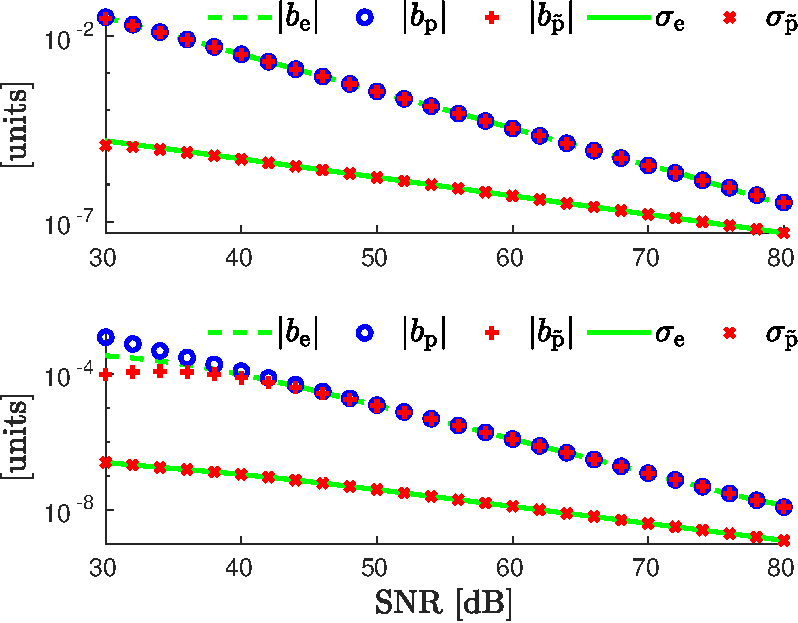
\includegraphics[width=0.69\columnwidth]{./ChapterStatisticalAnalysis/fig/Fig_1.pdf} 
\caption{ \label{fig:y} \color{blue} The exact response of the model is used in the simulations of the two EIV problem types. For the structured EIV problem, it is important to consider the transient response. Thus, we use the first 200 samples. The dashed lines show the values of ${y}$ that are 2\% above and below the steady-regime output value\color{black}. } 
\end{figure}

\color{black}

%In the structured EIV problem the perturbation $\mathbf{E}$ is correlated with $\bm{\epsilon}$.
The MC simulations performed $N_{MC} = 10^6$ runs of the LS solver with different realizations of the additive perturbations $[\begin{matrix} \mathbf{E} & \bm{\epsilon}] \end{matrix}$.
The perturbation variance \color{blue} $\sigma_{\bm{\epsilon}}^2$ \color{black} was selected to have a signal-to-noise ratio (SNR) in the interval [30 dB, 80 dB], according to 
\begin{equation} \mathrm{SNR} = 20 \log_{10}{ \dfrac{ \sqrt{ \dfrac{1}{\color{blue}N\color{black}} \sum\limits_{t=1}^{\color{blue}N\color{black}}{ y(t)^2 } } }{ \sigma_{ \bm{\epsilon}}} } . \label{eqn:SNR} \end{equation} 

The constraint $\| \mathbf{M} \| < 1$ and the Taylor series expansion  (\ref{eqn:TseriesExp}) hold for SNR sufficiently high, and 
in this conditions, the derived expressions \color{blue} predict \color{black} the LS estimation bias and variance.
Thus, it is relevant to monitor the evolution of the largest $\mathbf{M}$ eigenvalue to detect the lower limit of the SNR  that allows the validity of the predictions.

The MC simulations provide empirical values of the bias and variance, through the sample mean and sample variance of the LS estimate $\widehat{\bm{\theta}}$.
The results presented in this Section focus the interest in the first element of $\widehat{\bm{\theta}}$, because in the structured EIV problem, the step input estimate is $\widehat{u} = \widehat{\bm{\theta}}_{\left[1\right]}$.

\subsection{Monte Carlo simulation results for an unstructured EIV problem with uncorrelated perturbations}

The MC simulation of the unstructured EIV problem solution was conducted using the following settings.
The perturbations $\mathbf{E}$ and $\bm{\epsilon}$ are normally distributed with zero mean and variances $\sigma_{\mathbf{E}}^2 = 2 \sigma_{\bm{\epsilon}}^2$.
\color{blue} 
This relationship between the variances is also present in the structured EIV problem, and then we have similar assumptions.
However, for the uncorrelated and unstructured EIV case, the perturbations $\mathbf{E}$ and $\bm{\epsilon}$ are independent.\color{black}

%In the following results we focus our interest in the first element of the estimate $\widehat{\bm{\theta}}$.


The difference between the sample mean of the estimate $\widehat{\bm{\theta}}_{\left[1\right]}$ and its true value $\bm{\theta}_{\left[1\right]}$ is the empirical bias $b_\mathrm{e}$.
\begin{equation} {b}_\mathrm{e} = \frac{1}{N_{\mathrm{MC}}} \sum_{i=1}^{N_{\mathrm{MC}}}{ \left( \widehat{\bm{\theta}}_{\left[1\right]} \right)_i -  \bm{\theta}_{\left[1\right]} } \approx \mu \left( \widehat{\bm{\theta}}_{\left[1\right]} \right) - \bm{\theta}_{\left[1\right]} . \end{equation}
The standard deviation of the estimate $\widehat{\bm{\theta}}_{\left[1\right]}$ is used to obtain the standard error $\sigma_\mathrm{e,err}$ of the MC simulation, which decreases with respect to the square root of the number of MC runs $N_{\mathrm{MC}}$ as it is explained in \citet{Hammersley75}: 
\begin{equation} \sigma_\mathrm{e,err} = \frac{ \sigma_\mathrm{e} \left( \widehat{\bm{\theta}}_{\left[1\right]} \right) }{\sqrt{N_{\mathrm{MC}}}}, \quad \mathrm{where} \quad \sigma_\mathrm{e}^2 \left( \widehat{\bm{\theta}}_{\left[1\right]} \right) = \frac{1}{N_{\mathrm{MC}}-1} \sum_{i=1}^{N_{\mathrm{MC}}}{ \left( \left( \widehat{\bm{\theta}}_{\left[1\right]} \right)_i - \mu \left( \widehat{\bm{\theta}}_{\left[1\right]} \right) \right)^2 } . \label{eqn:stderr} \end{equation}

In each of the $N_{\mathrm{MC}}$ runs we also obtain the aproximations of the estimation bias $\mathbf{b}_{\widetilde{\mathrm{p}} \left[1\right]}$ and variance $\mathbf{C}_{\widetilde{\mathrm{p}} \left[1,1\right]}$  from observed data, using Equations (\ref{eqn:biasEuST}), and (\ref{eqn:varEuST}).
Similarly as before, we get the sample mean of the aproximations to have bias and variance predictions from observed data 
 \begin{equation} b_{\widetilde{\mathrm{p}}} = \frac{1}{N_{\mathrm{MC}}} \sum_{i=1}^{N_{\mathrm{MC}}}{ \left( \mathbf{b}_{\widetilde{\mathrm{p}} \left[1\right]} \right)_i } , \quad \mathrm{and} 
 \quad v_{\widetilde{\mathrm{p}}}  = \frac{1}{N_{\mathrm{MC}}} \sum_{i=1}^{N_{\mathrm{MC}}}{ \left( \mathbf{C}_{\widetilde{\mathrm{p}} \left[1,1\right]} \right)_i } . \end{equation} 
The standard error of the bias prediction $b_{\widetilde{\mathrm{p}}}$ is given by
\begin{equation} \sigma_{\widetilde{\mathrm{p}}, \mathrm{err}} = \sqrt{ \frac{1}{N_{\mathrm{MC}} \left( N_{\mathrm{MC}}-1 \right)} \sum_{i=1}^{N_{\mathrm{MC}}} { \left( \left( \mathbf{b}_{\widetilde{\mathrm{p}} \left[1\right]} \right)_i - b_{\widetilde{\mathrm{p}}} \left( \widehat{\bm{\theta}}_{\left[1\right]} \right) \right)^2 } } . \end{equation}

The predicted bias $b_{\mathrm{p}} = \mathbf{b}_{\mathrm{p} \left[1\right]}$ and variance $v_{\mathrm{p}} = \mathbf{C}_{\mathrm{p} \left[1,1\right]}$ from exact data are obtained with one evaluation of the expressions (\ref{eqn:biasEu}) and (\ref{eqn:varEu}). %for unstructured EIV problems, or expressions (\ref{eqn:biasST}) and (\ref{eqn:varST}) for the structured EIV problem.

Figure \ref{fig:bias_sigma_NMC_unstr_str_n2} shows the empirical bias and the bias predictions, with their corresponding standard errors, \color{blue} for the unstructured EIV problem\color{black}.
The simulation settings for the structured and correlated EIV problem are described in the following subsection.
In the figure, it can be observed that the empirical bias $b_\mathrm{e}$ is proportional to the perturbation noise variance while the standard error $\sigma_\mathrm{e, err}$ is proportional to the perturbation noise standard deviation.
The bias predictions $b_\mathrm{p}$ and $b_{\widetilde{\mathrm{p}}}$ are accurate since they coincide with the empirical bias $b_\mathrm{e}$ in all the SNR interval for unstructured EIV problems. 
In both unstructured and structured EIV cases, the standard errors of the MC estimates $\sigma_{\mathrm{e, err}}$ and $\sigma_{\widetilde{\mathrm{p}}, \mathrm{err}}$ are smaller than the bias estimates $b_{\mathrm{e}}$ and $b_{\widetilde{\mathrm{p}}}$.
The bias estimates are spread near their sample means. 
The uncertainty is smaller than the bias, therefore, the MC simulation is meaningful.

\begin{figure}[htb!]
 \centering
 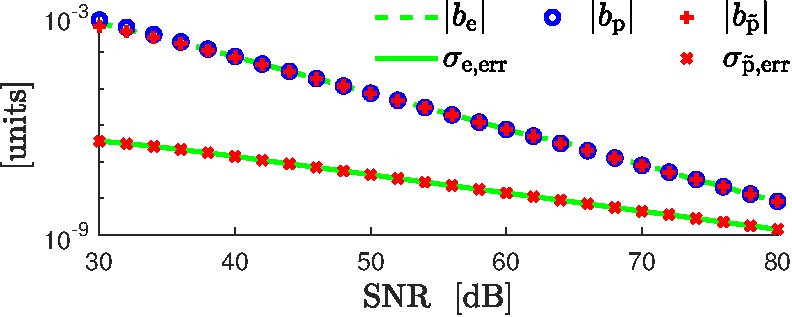
\includegraphics[width=0.69\columnwidth]{./ChapterStatisticalAnalysis/fig/Fig_2.pdf} 
  \caption{ \label{fig:bias_sigma_NMC_unstr_str_n2} 
  We observe the results of the LS solutions \color{blue} for the unstructured EIV problem\color{black}. These results are the empirical bias $b_{\mathrm{e}}$, the predicted bias from exact data $b_{\mathrm{p}}$, the predicted bias from observed data $b_{\widetilde{\mathrm{p}}}$, the empirical standard error $\sigma_{\mathrm{e, err}}$, and the standard error from the estimations using observed data $\sigma_{\widetilde{\mathrm{p}}, \mathrm{err}}$. The estimation biases are proportional to the perturbation variance and the estimation standard errors are proportional to the perturbation standard deviation. Since the standard errors are smaller than the biases, the MC simulation is meaningful. }
\end{figure}

The absolute and relative errors between the predicted and the empirical bias are shown in Figure \ref{fig:b_bt_abse_rele_unstr_e7}. 
The absolute errors decrease with respect to the perturbation variance.
The relative errors are lower than 5\% for SNR between 30 dB and 70 dB. 
There is an increment in the relative errors for SNR above 55 dB. 
 As the SNR increases, the empirical and the predicted bias decrease, as well as the bias error between them.
In order to reveal the bias error, more Monte Carlo runs are needed to reduce the uncertainty of the Monte Carlo simulation that depends on the square root of $N_{\mathrm{MC}}$, see Equation (\ref{eqn:stderr}).
If $N_{\mathrm{MC}}$ is insufficient, the uncertainty of the Monte Carlo simulation hides the bias error and we see this increasing effect of the relative errors. 

\begin{figure}[htb!]
  \centering
  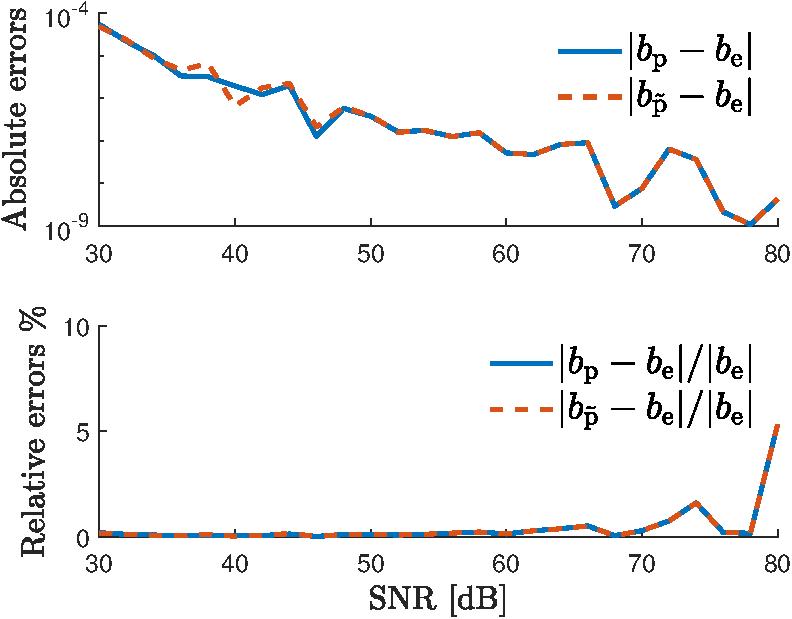
\includegraphics[width=0.69\columnwidth]{./ChapterStatisticalAnalysis/fig/Fig_3.pdf} 
  \caption{ \label{fig:b_bt_abse_rele_unstr_e7} The MC simulation shows that when we solve an unstructured EIV problem with LS, the absolute errors (top) between the predicted bias and the empirical bias are proportional to the perturbation noise variance as it is expected, and the relative errors (bottom) are smaller than 5\% for SNR below 70 dB. The bias prediction computed from exact data ${b}_\mathrm{p}$ is very similar to that computed using observed data $b_{\widetilde{\mathrm{p}}}$. } 
\end{figure}

The errors between the predicted and the empirical variance are shown in Figure \ref{fig:v_vt_abse_rele_unstr_e7}.
The absolute and relative errors decrease with respect to the perturbation variance.
The relative errors are lower than 5\% for SNR above 40 dB. 

\begin{figure}[htb!]
  \centering
  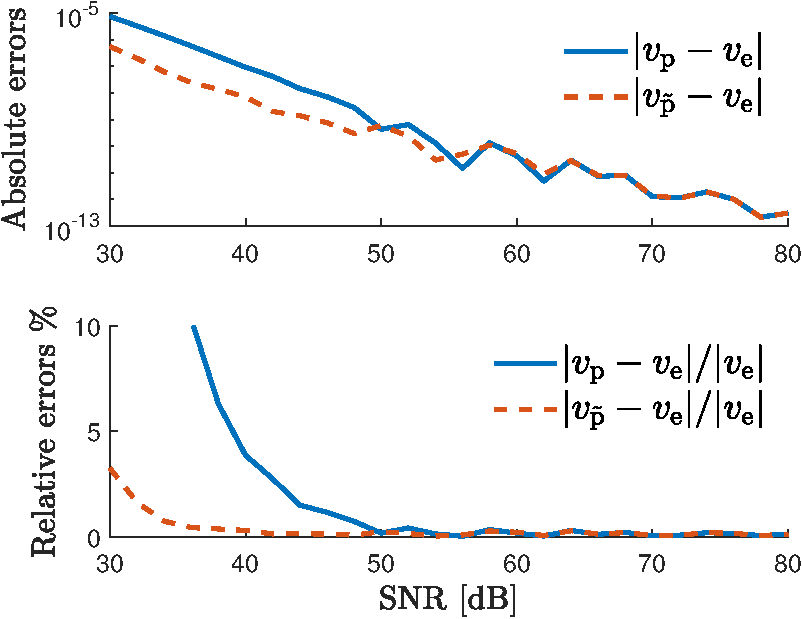
\includegraphics[width=0.69\columnwidth]{./ChapterStatisticalAnalysis/fig/Fig_4.pdf} 
  \caption{ \label{fig:v_vt_abse_rele_unstr_e7} The MC simulation shows that when we solve an unstructured EIV problem with LS, the absolute errors (top) between the predicted variances and the empirical variance are proportional to the perturbation noise variance, and the relative errors (bottom) are smaller than 5\% for SNR higher that 40 dB. The variance prediction computed using exact data ${v}_\mathrm{p}$ is very similar to that computed from observed data $v_{\widetilde{\mathrm{p}}}$. } 
\end{figure}

Figure \ref{fig:bv_btvt_abse_rele_unstr_e7} shows the absolute and the relative errors between the predictions computed from observed data and those computed from exact data.
The absolute errors between both predictions are proportional to the perturbation noise variance.
The bias and variance predictions, from either exact data or observed data, are equivalent for SNR above 35 dB since the relative errors are lower than 5\%.
The substitution of observed data on the prediction formulas is a valid procedure that allows the prediction of the estimate statistics.

\begin{figure}[htb!]
  \centering
  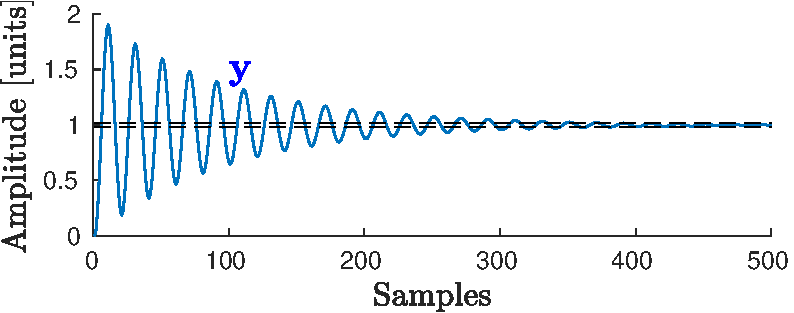
\includegraphics[width=0.69\columnwidth]{./ChapterStatisticalAnalysis/fig/Fig_5.pdf} 
  \caption{ \label{fig:bv_btvt_abse_rele_unstr_e7} The MC simulation shows that when we solve an unstructured EIV problem with LS, the absolute errors (top) between the prediction with observed data and the prediction with exact data are proportional to the perturbation noise variance. The use of observed data instead of exact data in the prediction formulas is valid when the SNR is above 35 dB since the relative errors (bottom) are smaller than 5\%. } 
\end{figure}


\subsection{Monte Carlo simulation results for a structured EIV problem with correlated perturbations}

\color{blue}The MC simulation of the structured EIV problem (\ref{eqn:ddsiemnd}) solution was conducted using the step response $\widetilde{{y}}$ of the sensor model (\ref{eqn:msdst}).
We use the same exact data response as for the previous subsection, but in this case the perturbations of the regression matrix $\widetilde{\mathbf{K}}$ have Hankel structure and are correlated with the perturbations of the regressor vector $\widetilde{\mathbf{y}}$.
The perturbations $\bm{\epsilon}$ are normally distributed with zero mean and variance $\sigma_{\bm{\epsilon}}^2$, and are also used to build the perturbations $\mathbf{E}$.
Due to the Hankel structure in Equation (\ref{eqn:matrixE}), the variances of the perturbations $\mathbf{E}$ and $\bm{\epsilon}$ are related by $\sigma_{\mathbf{E}}^2 \approx 2 \sigma_{\bm{\epsilon}}^2$.

The spectral radius of the matrix $\mathbf{K}$ in Equation (\ref{eqn:TseriesExp}) is observed for the SNR values in the interval of interest.
As can be observed in Figure \ref{fig:spectral_radius}, for SNR values larger than 35 dB, the perturbation levels make the spectral radius $\| \mathbf{M} \| < 1$, and, therefore, ensure the approximation given by the Taylor series expansion of the inverse matrix. 
Below an SNR of 35 dB, the spectral radius of $\mathbf{K}$  grows above 1. 
In the rest of this subsection we will evaluate the effect of the error introduced by the approximation.

\begin{figure}[htb!]
 \centering
 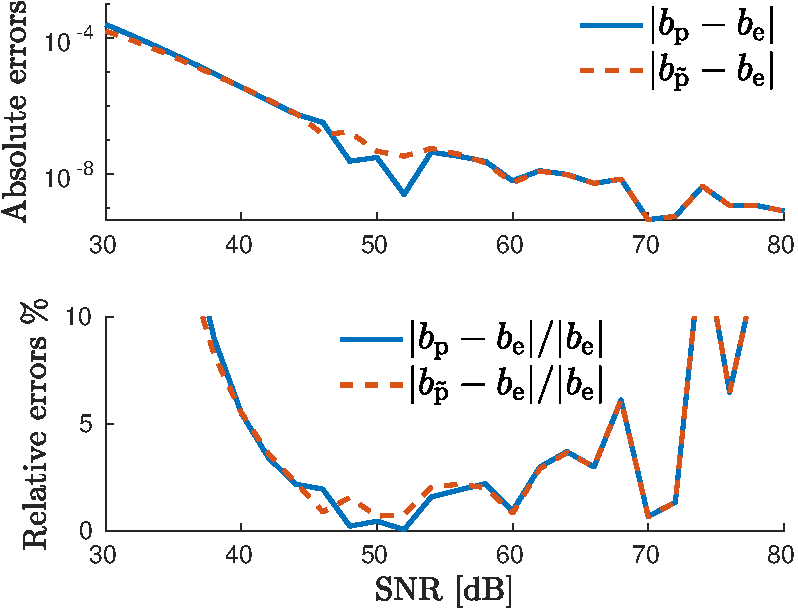
\includegraphics[width=0.69\columnwidth]{./ChapterStatisticalAnalysis/fig/Fig_6.pdf} 
  \caption{ \label{fig:spectral_radius} 
  \color{blue} The spectral radius $\| \mathbf{M} \|$ is evaluated for different perturbation levels. The approximation of the inverse matrix with the Taylor series expansion gives small error when $\| \mathbf{M} \| < 1$. The SNR values that increase the spectral radius above one are those below 35 dB\color{black}. }
\end{figure}


We are interested in the mean-squared error of the of the step input estimation, obtained empirically with the Monte Carlo simulation\color{black}.
The empirical bias is the sample mean of the $N_{\mathrm{MC}}$ estimates minus the true value
 \begin{equation} {b}_\mathrm{e} = \frac{1}{N_{\mathrm{MC}}} \sum_{i=1}^{N_{\mathrm{MC}}}{ \widehat{u}_i - u } \approx \mu \left( \widehat{u} \right) - u. \end{equation}
The standard error associated to this empirical bias estimation is defined in \citet{Hammersley75} as 
\begin{equation} \sigma_\mathrm{e, err} = \frac{\sigma_\mathrm{e} \left( \widehat{u} \right) }{\sqrt{N_{\mathrm{MC}}}}, \quad \mathrm{where} \quad \sigma_\mathrm{e}^2 \left( \widehat{u} \right) = \frac{1}{N_{\mathrm{MC}}-1} \sum_{i=1}^{N_{\mathrm{MC}}}{ \left( { \widehat{u}}_i - \mu \left( \widehat{u} \right) \right)^2 } . \end{equation} 

The plots \color{blue} in \color{black} Figure \ref{fig:bias_sigma_NMC_str_str_n2} show the empirical bias, the bias predictions (\ref{eqn:biasE}) and (\ref{eqn:biasST}), and their corresponding standard errors, for the structured EIV problem.
The empirical bias $b_\mathrm{e}$ is proportional to the perturbation noise variance, and
the bias predictions $b_\mathrm{p}$ and $b_{\widetilde{\mathrm{p}}}$ coincide with the empirical bias $b_\mathrm{e}$ only for SNR above 40 dB.
This indicates that the SNR drops to a point where the constraint $\| \mathbf{M} \| < 1$ is no longer satisfied.
At an SNR of 30 dB the perturbation noise affects the bias prediction from observed data and it is three times smaller than the empirical bias.

\begin{figure}[htb!]
 \centering
 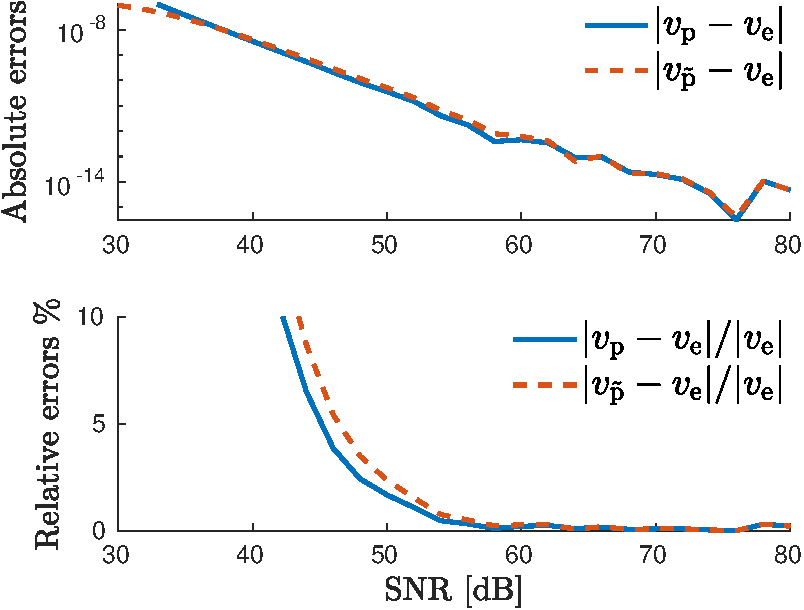
\includegraphics[width=0.69\columnwidth]{./ChapterStatisticalAnalysis/fig/Fig_7.pdf} 
  \caption{ \label{fig:bias_sigma_NMC_str_str_n2} 
  We observe the results of the LS solutions \color{blue} for the structured EIV problem\color{black}. These results are the empirical bias $b_{\mathrm{e}}$, the predicted bias from exact data $b_{\mathrm{p}}$, the predicted bias from observed data $b_{\widetilde{\mathrm{p}}}$, the standard error $\sigma_{\mathrm{e,err}}$ of the empirical bias, and the standard error $\sigma_{\widetilde{\mathrm{p}} \mathrm{,err}}$ of the the estimations bias computed using observed data. The estimation biases are proportional to the perturbation variance and the estimation standard errors are proportional to the perturbation standard deviation. Since the standard errors are smaller than the biases, the MC simulation is meaningful. }
\end{figure}

The absolute and relative errors between the predicted and the empirical bias are shown in Figure \ref{fig:b_bt_abse_rele_str_e7}.
It can be seen that the absolute errors are proportional to the perturbation variance, and the relative errors are lower than 5\% for SNR higher than 40 dB. 
%Nevertheless, the perturbation SNR in practical applications is not high and is near 40 dB


\begin{figure}[htb!]
  \centering
  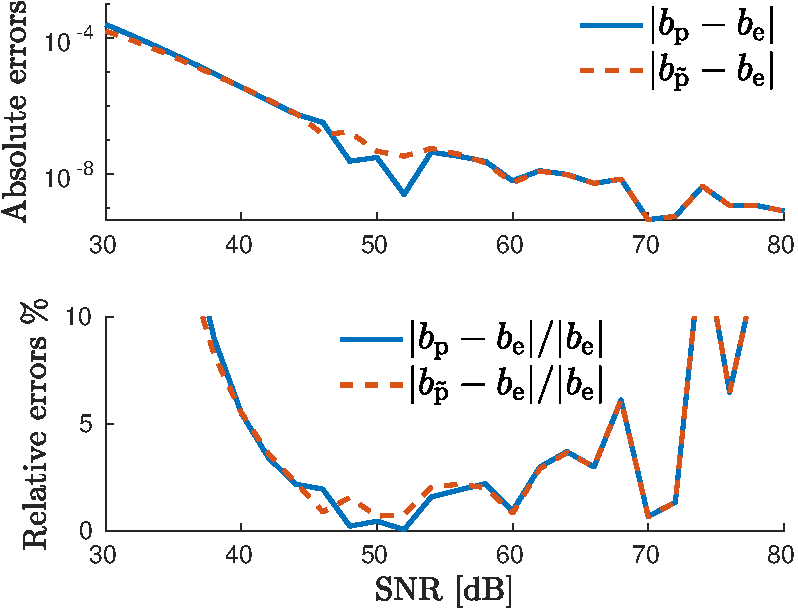
\includegraphics[width=0.69\columnwidth]{./ChapterStatisticalAnalysis/fig/Fig_8.pdf} 
  \caption{ \label{fig:b_bt_abse_rele_str_e7} The MC simulation shows that when we solve a structured EIV problem with LS, the absolute errors (top) between the predicted bias and the empirical bias $b_{\mathrm{e}}$ are proportional to the perturbation noise variance, and the relative errors (bottom) are smaller than 5\% only for SNR above 40 dB.}
\end{figure}


The absolute and relative errors between the empirical and the predicted variance, equations (\ref{eqn:varE}) and (\ref{eqn:varST}), are shown in Figure \ref{fig:v_vt_abse_rele_str_e7}.
These absolute errors are proportional to the perturbation noise variance, whereas
the relative errors are lower than 5\% for SNR higher than 45 dB. 

The absolute and relative errors between the two predictions from observed data and from exact data, are shown in Figure \ref{fig:bv_btvt_abse_rele_str_e7}.
These absolute errors are also proportional to the perturbation noise variance, and
the relative errors show that the bias and variance predictions from either of the two alternatives are equivalent for SNR higher than 45 dB.

\begin{figure}[htb!]
  \centering
  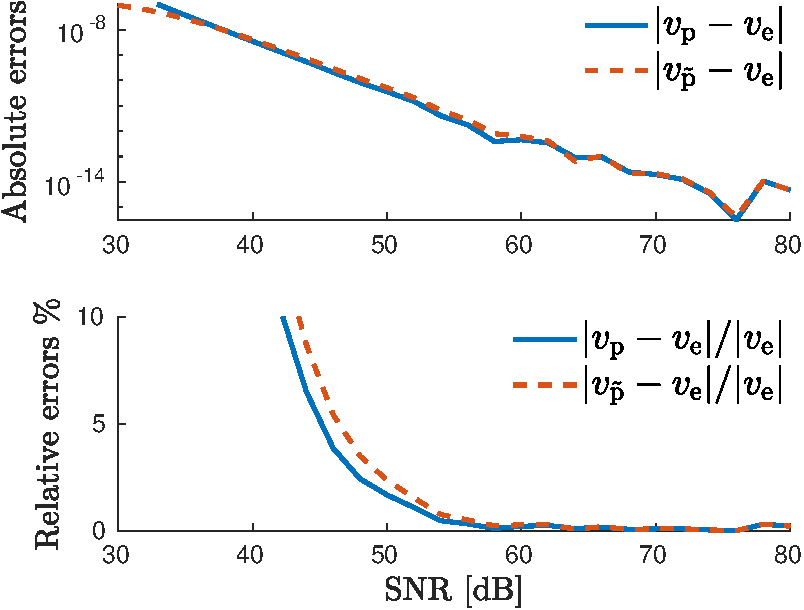
\includegraphics[width=0.69\columnwidth]{./ChapterStatisticalAnalysis/fig/Fig_9.pdf} 
  \caption{ \label{fig:v_vt_abse_rele_str_e7} The MC simulation shows that when we solve a structured EIV problem with LS, the absolute errors (top) between the predicted and the empirical variance are proportional to the perturbation variance, and the relative errors (bottom) between the predicted and the empirical variance are smaller than 5\% for SNR above 45 dB. }
\end{figure}

\begin{figure}[htb!]
  \centering
  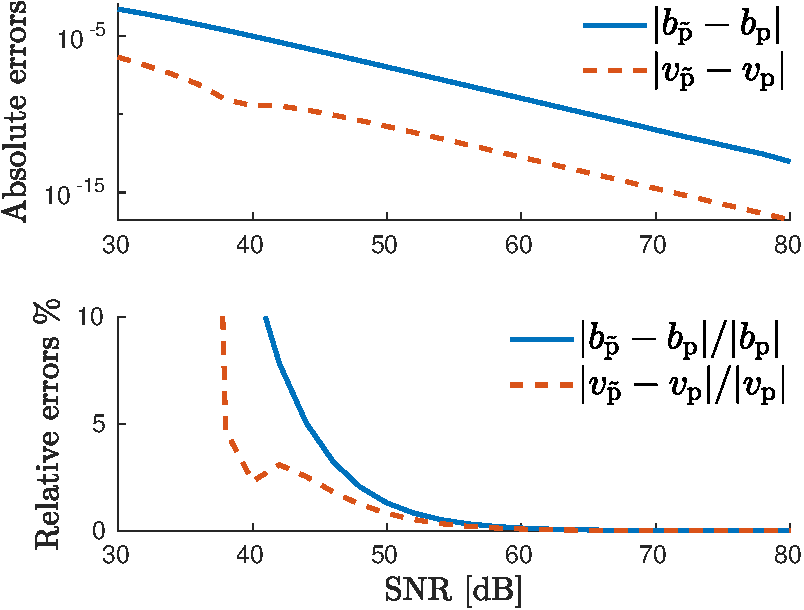
\includegraphics[width=0.69\columnwidth]{./ChapterStatisticalAnalysis/fig/Fig_10.pdf} 
  \caption{ \label{fig:bv_btvt_abse_rele_str_e7} The MC simulation shows that when we solve a structured EIV problem with LS, the absolute errors (top) between the predictions computed from observed data and those from exact data are proportional to the perturbation noise variance. According to the relative errors (bottom), the substitution is valid for SNR higher than 45 dB. } 
\end{figure}

The simulation results show that the LS solution of the structured and correlated EIV problem is more sensitive to the perturbation.
This represents a low limit in the SNR interval imposed by the noise level.
In practical applications it is common to have SNRs of 40 dB and the user needs to be aware of the prediction error that the method has.
We measure this prediction error with the mean squared error (MSE), defined as
\begin{equation} \mathrm{MSE} = \sigma^2 + b^2. \end{equation}
 By comparing the different MSEs to the CRLB of the structured EIV problem,
Figure \ref{fig:MSE_CRLB_str_stat} shows that the MSEs has the same proportionality as the CRLB with respect to the disturbing noise variance.
The MSEs are three times larger than the CRLB.
Since the difference between $\mathrm{MSE}_{\widetilde{\mathrm{p}}}$ and the CRLB is lower than one order of magnitude, 
the LS estimation of the structured EIV problem produces results that are comparable to the ML estimation.
The $\mathrm{MSE}_{\widetilde{\mathrm{p}}}$ computed from observed data approaches the CRLB for SNR below 40 dB.
This is due to the constraint violation of the Taylor series expansion.


\begin{figure}[!htpb]
  \centering
  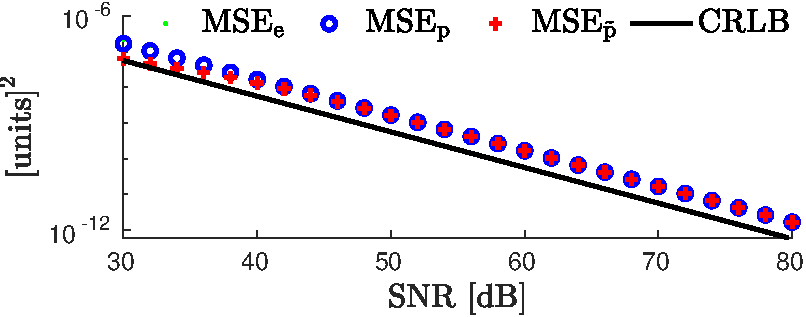
\includegraphics[width=0.69\columnwidth]{./ChapterStatisticalAnalysis/fig/Fig_11.pdf}
  \caption{\label{fig:MSE_CRLB_str_stat}
The mean squared errors of the LS estimate are close to the Cram\'er-Rao lower bound. This is a positive indication of the goodness of the LS estimator for the structured EIV problem. The mean squared error of the empirical estimates is represented by $\mathrm{MSE}_{\mathrm{e}}$, and those of the predictions are $\mathrm{MSE}_{\mathrm{p}}$ and $\mathrm{MSE}_{\widetilde{\mathrm{p}}}$. The $\mathrm{MSE}_{\widetilde{\mathrm{p}}}$ is smaller than CRLB below 40 dB of SNR because of the introduced bias error, but the difference between $\mathrm{MSE}_{\widetilde{\mathrm{p}}}$ and the CRLB is lower than one order of magnitude.}
\end{figure}

\color{blue}

\subsection{Simulation results observed when the perturbation noise does not concord with the type of perturbation assumed by the derived expressions}

In this section, the numerical study of the expressions that calculate the step input estimation bias and variance considers the situation when the perturbation noise is not in agreement with the assumptions made during the analysis and the derivation of the predicting expressions.  
In other words, the unstructured perturbation is used in the expressions derived for the structured case, and the structured perturbation is used in the expressions derived for the unstructured case. 
Two Monte Carlo simulations, each one with $N_{MC} = 10^6$ runs, were conducted and the relevant results are illustrated in Figures \ref{fig:unstrFormula_strData} and \ref{fig:strFormula_unstrData}. 
It is expected that the performance in these conditions is very far from that obtained when using the expressions in concordance with the perturbation type they were derived for.
The results confirm this argument, since the relative errors are in general close to 100\%.
An exception is the variance prediction computed with the formulas derived for the unstructured case, but using structured perturbation. 
Only in this combination, the relative error of the variance prediction is aroun 10\% for SNR below 70 dB.


\begin{figure}[!htpb]
  \centering
  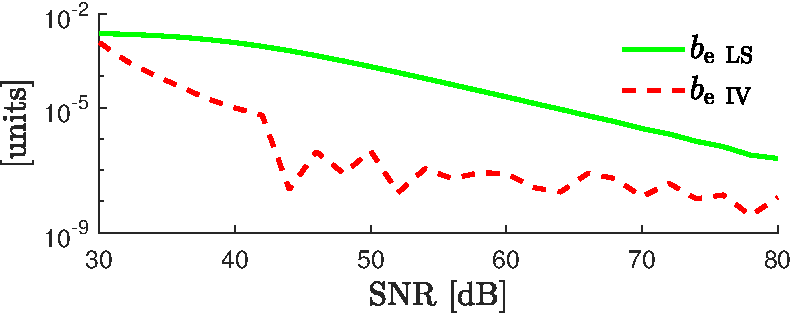
\includegraphics[width=0.69\columnwidth]{./ChapterStatisticalAnalysis/fig/Fig_12.pdf}
  \caption{\label{fig:unstrFormula_strData} \color{blue} We observe the results obtained from the Monte Carlo simulation, when the perturbation noise is structured and we use the predicting expressions that were derived assuming the perturbation noise is unstructured. A comparison of the empirical and the predicted bias and variance of the input estimation shows that the prediction formulas fail, since the relative errors between the empirical and the predicted statistical moments are larger than 10\%.}
\end{figure}

\begin{figure}[!htpb]
  \centering
  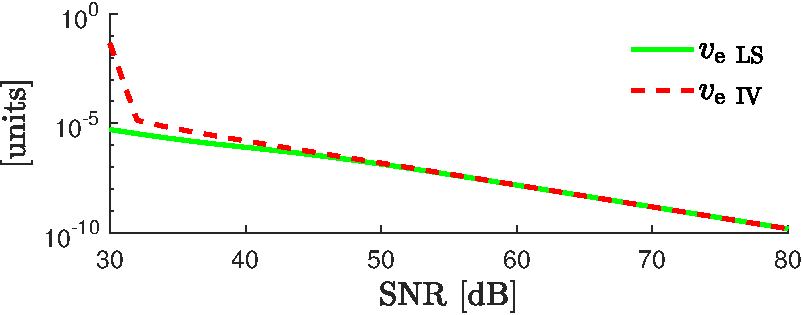
\includegraphics[width=0.69\columnwidth]{./ChapterStatisticalAnalysis/fig/Fig_13.pdf}
  \caption{\label{fig:strFormula_unstrData} \color{blue} We observe the results obtained from the Monte Carlo simulation, when the perturbation noise is unstructured and we use the prediction expressions that were derived assuming the perturbation noise is structured. A comparison of the empirical and the predicted bias and variance of the input estimation shows that in these conditions, the derived expressions fail to predict the statistical moments. If the perturbation noise does not have the structure assumed by the prediction expressions, the relative error remains high above 10\% in all the SNR interval. }
\end{figure}



\subsection{Simulation results for the structured IV solution}

The structured IV problem, with instrumental variable (\ref{eqn:matrixZ_t}), and normal equations (\ref{eqn:neq_siv}), admits also a recursive least-squares solution. 
A Monte Carlo simulation was conducted to find the empirical bias and variance of the solution to the IV problem.
This simulation is conducted using the same conditions as for the structured EIV problem, in the previous subsection, and aims to compare the EIV and the IV problem solutions.   
In Figure \ref{fig:bvMSE_IV} we can observe, for different SNR levels, the empirical bias (top), variance(center), and mean-squared error (bottom) of the solutions to the EIV and the IV problems.
The empirical bias the IV solution is two orders of magnitude smaller than that of the EIV solution. 
Nevertheless, the empirical variance of the two solutions are very close together, making the mean-squared error almost identical.
 

\begin{figure}[!htpb]
  \centering
  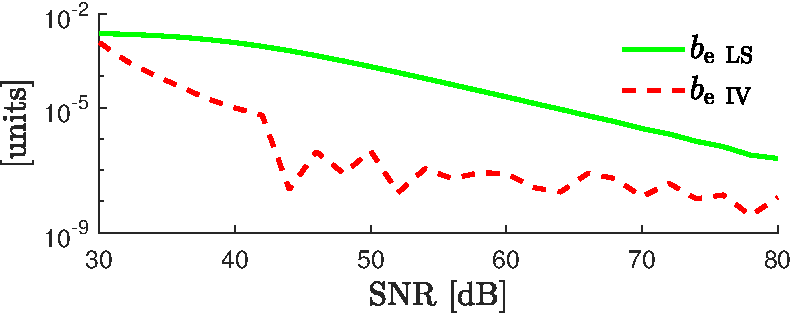
\includegraphics[width=0.69\columnwidth]{./ChapterStatisticalAnalysis/fig/Fig_14.pdf}
  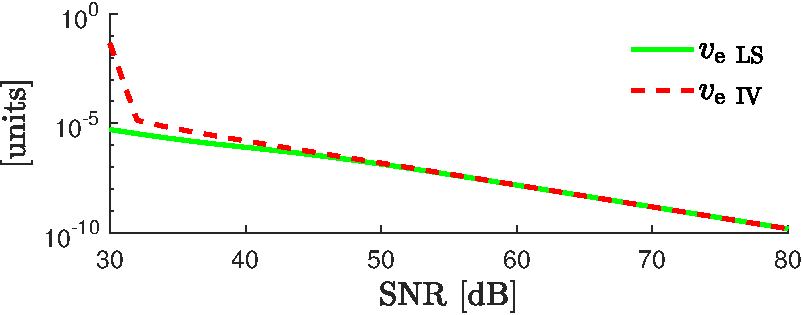
\includegraphics[width=0.69\columnwidth]{./ChapterStatisticalAnalysis/fig/Fig_15.pdf}
  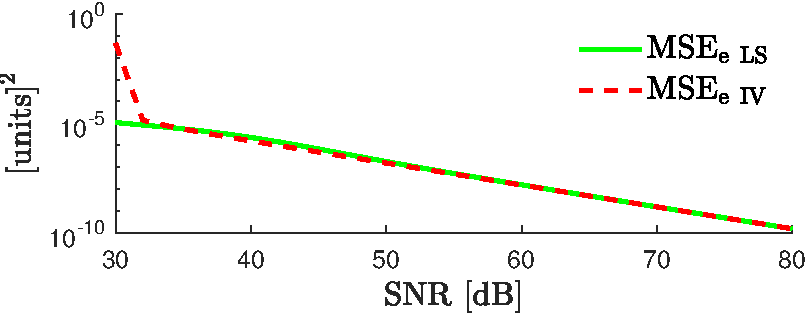
\includegraphics[width=0.69\columnwidth]{./ChapterStatisticalAnalysis/fig/Fig_16.pdf}
  \caption{\label{fig:bvMSE_IV} \color{blue} In a simulation, the solutions of the structured EIV and IV problems are empirically compared. The bias from solving the IV problem is noticeable smaller, by two orders of magnitude, than the one from solving the EIV problem. This argument is valid for SNRs higher that 35 dB. The obtained variances, on the other hand, are very similar in the same SNR interval. As a consequence, the mean-squared errors almost coincide.}
\end{figure}


\color{black}


\section{Conclusions}

We conducted a statistical analysis of a structured errors-in-variables (EIV) estimation problem with correlation to find the first and second moments of its least-squares solution.
This estimation problem occurs in metrology when we estimate the value of a measurand directly from the sensor transient response.
The data-driven estimation of the physical quantity is formulated as a structured EIV problem with correlation that uses the observed transient response to construct both the regression matrix and the regressor.
The real-time implementation of the method uses a recursive least-squares algorithm that is simple and has low computational complexity.
The assessment of the uncertainty is done using the estimation bias and variance.

The conducted statistical analysis produced expressions that predict the estimation bias and variance for given sample size and perturbation level of the observed response.
The Monte Carlo simulation validated the predictions.
We compared the results of solving an unstructured and uncorrelated EIV problem with a structured and correlated EIV problem to understand how the structure and the correlation impacts in the estimation.
We found that the predictions in the structured case are more susceptible to perturbations.
This is due to the two approximations involved, a second-order Taylor series expansion of the estimate, and the substitution of perturbed data on the prediction expressions.
The relative error results indicate that the estimation bias, and variance are predicted using the derived expressions, and the observed data.
The mean squared error of the estimate is close to the results of the maximum likelihood estimate given by the Cram\'er-Rao lower bound.

The bias and variance can be accurately predicted, provided that the Taylor series expansion is valid.
This constraint has to be taken into account to ensure the effectiveness of the method in practical applications.
In the example, it was observed that when the SNR lies outside the validity region, the bias and variance estimation was at most three times larger than the empirical values.

The methodology presented in this chapter can be applied to estimate the uncertainty of the solutions to other structured EIV problems.
The bias and variance expressions obtained after the statistical analysis depend on each specific structure.


\begin{comment}
\section{STATISTICAL ANALYSIS - Ramp input}

\subsubsection{Statistical analysis of the subspace method}

To obtain the first and second moments of the step input estimate $\widehat{u}$, we need to study the solution
\begin{equation} \widehat{\bm{\theta}} = ( \mathbf{K}^\top \mathbf{W} \mathbf{K}  )^{-1} \mathbf{K}^\top \mathbf{W} \mathbf{y} , \label{eqn:xhat} \end{equation}
of the overdetermined structured errors-in-variables EIV problem (\ref{eqn:min_ewrls}).
Using a second order Taylor series expansion of the inverse matrix we can approximate the LS solution as
\begin{equation} \widehat{\bm{\theta}} \approx \left( \mathbf{I} - \mathbf{M} + \mathbf{M}^2 \right) \mathbf{C}^{-1} (\widebar{\mathbf{K}} + \mathbf{E})^\top \mathbf{W} (\widebar{\mathbf{y}} + \bm{\epsilon}). \label{eqn:xhatexp} \end{equation} 
where 
\begin{equation} \widebar{\mathbf{C}} = \widebar{\mathbf{K}}^\top \mathbf{W} \widebar{\mathbf{K}}, \quad \text{and} \quad \mathbf{M} = \widebar{\mathbf{C}}^{-1} ( \widebar{\mathbf{K}}^\top \mathbf{W} \mathbf{E} + \mathbf{E}^\top \mathbf{W} \widebar{\mathbf{K}} + \mathbf{E}^\top \mathbf{W} \mathbf{E} ). \end{equation} 

The Taylor series approximation of $\widehat{\bm{\theta}}$ enables the calculation of the estimation bias and covariance since the measurement noise $\bm{\epsilon}$ and $\mathbf{E}$ are no more subject to matrix inversion. 
The bias and the covariance of the estimate $\widehat{\bm{\theta}}$ are obtained from
\begin{equation}  \mathbf{b} \left(\widehat{\bm{\theta}} \right) = \mathbf{\mu} - \widebar{\bm{\theta}}, \label{eqn:biasdef} \end{equation}
\begin{equation} \begin{aligned} \mathrm{\mathbf{Cov}} \left( \widehat{\bm{\theta}} \right) & = \mathbb{E} \left\{ \left( \widehat{\bm{\theta}} - \mathbf{\mu} \right)  \left( \widehat{\bm{\theta}} - \mathbf{\mu} \right)^\top \right\} . \end{aligned} \label{eqn:covdef} \end{equation} 
where $\mathbf{\mu} = \mathbb{E} \left\{ \widehat{\bm{\theta}} \right\}$ is the expected value of the estimate and $\widebar{\bm{\theta}}$ is the true value. 
Considering the structure of the EIV problem, the bias and the covariance of the estimate approximation (\ref{eqn:xhatexp}) can be expressed as
\begin{equation} \begin{aligned} \widebar{\mathbf{b}}_{\mathrm{p}} \left( \widehat{x} \right) & \approx \widebar{\mathbf{C}}^{-1} \left(  \left( \widebar{\mathbf{K}}^\top \mathbf{W} \widebar{\mathbf{B}}_1 - \widebar{\mathbf{B}}_2 \right) \bm{\theta} - \left( \widebar{\mathbf{K}}^\top \mathbf{W} \widebar{\mathbf{B}}_3 - \widebar{\mathbf{B}}_4 \right) \right), \end{aligned} \label{eqn:biasE} \end{equation}
\begin{equation} \begin{aligned} \widebar{\mathrm{\mathbf{Cov}}}_{\mathrm{p}} \left( \widehat{\bm{\theta}} \right) & \approx \widebar{\mathbf{K}}^\dagger \mathbf{W} \left( \sigma_{\epsilon}^2 \mathbf{I}_{T-n} + \widebar{\mathbf{C}}_1 - \widebar{\mathbf{C}}_2 - \widebar{\mathbf{C}}_2^\top \right) \mathbf{W} \widebar{\mathbf{K}}^{\dagger \top}  - \widebar{\mathbf{b}}_{\mathrm{p}} \left( \widehat{x} \right) \widebar{\mathbf{b}}_{\mathrm{p}}^\top \left( \widehat{x} \right), \end{aligned} \label{eqn:varE} \end{equation}
where $\widebar{\mathbf{B}}_1 = \mathbb{E} \Big\{ \mathbf{E} \widebar{\mathbf{K}}^\dagger \mathbf{W} \mathbf{E} \Big\}$, $\widebar{\mathbf{B}}_2 = \mathbb{E} \Big\{ \mathbf{E}^\top \mathbf{W} \widebar{\mathbf{P}}_\perp \mathbf{E} \Big\}$, $\widebar{\mathbf{B}}_3 = \mathbb{E} \Big\{ \mathbf{E} \widebar{\mathbf{K}}^\dagger \mathbf{W} \bm{\epsilon} \Big\}$, $\widebar{\mathbf{B}}_4 = \mathbb{E} \Big\{ \mathbf{E}^\top \mathbf{W} \widebar{\mathbf{P}}_\perp \bm{\epsilon} \Big\}$, $\widebar{\mathbf{C}}_1 = \mathbb{E} \Big\{ \mathbf{E} \bm{\theta} \bm{\theta}^\top \mathbf{E}^\top \Big\}$, \linebreak $\widebar{\mathbf{C}}_2 = \mathbb{E} \Big\{ \mathbf{E} \bm{\theta} \bm{\epsilon}^\top \Big\}$, $\widebar{\mathbf{P}}_\perp = \mathbf{I} - \widebar{\mathbf{K}} \widebar{\mathbf{K}}^\dagger \mathbf{W}$, and $\mathbf{K}^\dagger$ is the pseudo-inverse matrix of $\mathbf{K}$. 

The bias and covariance given by expressions (\ref{eqn:biasE}) and (\ref{eqn:varE}) depend on the unobservable true values $\widebar{\bm{\theta}}$ and $\widebar{\mathbf{K}}$.
The measured observations are in the sensor step response $\mathbf{y}$, and from its observations we construct $\mathbf{K}$ and compute $\widehat{\bm{\theta}}$.
The substitution of the measured data in the expressions gives an approximation of the estimation bias and covariance. 
We have then
\begin{equation} \begin{aligned} \mathbf{b}_{\mathrm{p}} \left( \widehat{\bm{\theta}} \right) & \approx \mathbf{C}^{-1} \left(  \left( \mathbf{K}^\top \mathbf{W} \mathbf{B}_1 - \mathbf{B}_2 \right) \widehat{\bm{\theta}} - \left( \mathbf{K}^\top \mathbf{W} \mathbf{B}_3 - \mathbf{B}_4 \right) \right), \end{aligned} \label{eqn:biasST} \end{equation}
  \begin{equation} \begin{aligned} {\mathrm{\mathbf{Cov}}}_{\mathrm{p}} \left( \widehat{\bm{\theta}} \right) & \approx \mathbf{K}^\dagger \mathbf{W} \left( \sigma_{\epsilon}^2 \mathbf{I}_{T-n} + \mathbf{C}_1 - \mathbf{C}_2 - \mathbf{C}_2^\top \right) \mathbf{W} \mathbf{K}^{\dagger \top} - \mathbf{b}_{\mathrm{p}} \left( \widehat{x} \right) \mathbf{b}_{\mathrm{p}}^\top \left( \widehat{x} \right), \end{aligned} \label{eqn:varST} \end{equation}
  where $\mathbf{B}_1 = \mathbb{E} \Big\{ \mathbf{E} \mathbf{K}^\dagger \mathbf{W} \mathbf{E} \Big\}$, $\mathbf{B}_2 = \mathbb{E} \Big\{ \mathbf{E}^\top \mathbf{W} \mathbf{P}_\perp \mathbf{E} \Big\}$, $\mathbf{B}_3 = \mathbb{E} \Big\{ \mathbf{E} \mathbf{K}^\dagger \mathbf{W} \bm{\epsilon} \Big\}$, $\mathbf{B}_4 = \mathbb{E} \Big\{ \mathbf{E}^\top \mathbf{W} \mathbf{P}_\perp \bm{\epsilon} \Big\}$, $\mathbf{C}_1 = \mathbb{E} \Big\{ \mathbf{E} \widehat{\bm{\theta}} \widehat{\bm{\theta}}^\top \mathbf{E}^\top \Big\}$, $\mathbf{C}_2 = \mathbb{E} \Big\{ \mathbf{E} \widehat{\bm{\theta}} \bm{\epsilon}^\top \Big\}$, and $\mathbf{P}_\perp = \mathbf{I} - \mathbf{K} \mathbf{K}^\dagger \mathbf{W}$. 

  The results of the expected values $\mathbf{B}_1$, $\mathbf{B}_2$, $\mathbf{B}_3$, $\mathbf{B}_4$, $\mathbf{C}_1$, and $\mathbf{C}_2$, were described by the authors of this paper in \citet{Quintana19}.
The bias and covariance were obtained to extend previous analysis conducted on EIV estimation problems without an imposed structure \citet{Vaccaro94, Stewart90SPT}.
It was shown that the bias and variance expressions (\ref{eqn:biasST}) and (\ref{eqn:varST}) are valid predictions of the first and second moments of the LS estimate of a Hankel structured EIV problem.
The problem formulated by the step input estimation method belongs to this type of structured EIV problems and can use the derived expressions to find the bias and variance of the input estimate $\widehat{u}$.
The bias of the estimate $\widehat{u}$ is the fist element of $\mathbf{b}_{\mathrm{p}} \left( \widehat{\bm{\theta}} \right)$ and the variance of $\widehat{u}$ is the first element in the main diagonal of $\mathrm{\mathbf{Cov}}_{\mathrm{p}} \left( \widehat{\bm{\theta}} \right)$.


\subsubsection{Cram\'er-Rao lower bound of the structured EIV problem}

To find the Cram\'er-Rao lower bound (CRLB) of the structured EIV estimation problem (\ref{eqn:min_ls}), we consider that this structured and correlated estimation problem can be expressed as a linear in the measurements problem \citet{Pintelon12Book}
\begin{equation} e (\widehat{\bm{\theta}}, \mathbf{z}) = \mathbf{M}_1( \widehat{\bm{\theta}} ) \ \mathbf{z} = \underbrace{\begin{bmatrix} \mathbf{I}_{T-n} & - \widehat{\bm{\theta}}^T \otimes \mathbf{I}_{T-n} \end{bmatrix}}_{\mathbf{M}_1( \widehat{\bm{\theta}} )} \underbrace{\begin{bmatrix} \mathbf{y} \\ \mathrm{vec} ( \mathbf{K} ) \end{bmatrix}}_{\mathbf{z}} = 0 . \label{eqn:M1vecyK} \end{equation}
where $\mathbf{z} = \widebar{\mathbf{z}} + \bm{\epsilon}_{\mathbf{z}}$.
To have the CRLB, it is necessary the existence of the true model $\mathbf{M}_1( \bm{\theta} ) \ \mathbf{z} = 0$.
The measurement perturbation $\bm{\epsilon}_{\mathbf{z}}$ is assumed to be normally distributed with covariance matrix $\mathbf{C}_{\mathbf{z}}$, and then, the loglikelihood function of the structured and correlated EIV problem is
\begin{equation} \ln{ l(\mathbf{z}, \widehat{\mathbf{z}}, \widehat{\bm{\theta}}) } = - \frac{1}{2} \left( \mathbf{z} - \widehat{\mathbf{z}} \right)^\top \mathbf{C}_{\mathbf{z}}^{-1} \left( \mathbf{z} - \widehat{\mathbf{z}} \right) + \mathrm{constant}, \end{equation}
where the elements of $\widehat{\mathbf{z}}$ are the estimated parameters of the measurements $\mathbf{z}$,  that satisfy $\mathbf{M}_1(\widehat{\bm{\theta}}) \ \widehat{\mathbf{z}} = 0$.
The size of the Fisher information matrix $\mathbf{Fi}(\bm{\theta}, \mathbf{z})$ depends on the number of unknowns in $\widehat{\mathbf{z}}$ and grows with the sample size.
However, the Fisher information matrix $\mathbf{Fi}(\bm{\theta})$ is obtained from $\mathbf{Fi}(\bm{\theta}, \mathbf{z})$, by doing inversion by parts \citet{Pintelon12Book} \S 19, and can be expressed as  
\begin{equation} \mathbf{Fi}(\bm{\theta}) = \left( \frac{\partial e (\widehat{\bm{\theta}}, \mathbf{z}) }{\partial \bm{\theta} } \right)^\top \left( \mathbf{M}_1( \bm{\theta} ) \mathbf{C}_{\mathbf{z}}  \mathbf{M}_1^\top( \bm{\theta} ) \right)^{-1}  \left( \frac{\partial e (\widehat{\bm{\theta}}, \mathbf{z}) }{\partial \bm{\theta} } \right) .
 \label{eqn:FIM}   \end{equation} 
The partial derivatives are evaluated at the true values $\bm{\theta}$. 
Thus, the covariance matrix of the measurements is

\begin{equation} \mathbf{C}_{\mathbf{z}} = \sigma_{\epsilon}^2 \begin{bmatrix} \mathbf{I}_{T-n} & \mathbf{0}_{T-n} & \mathbf{D}_1 \\ \mathbf{0}_{T-n} & \mathbf{0}_{T-n} & \mathbf{0}_{T-n \times n \left( T-n \right)}  \\  \mathbf{D}_1^\top & \mathbf{0}_{n \left( T-n \right) \times T-n} & \mathbf{D}_2  \end{bmatrix}  \label{eqn:Cz} \end{equation} 
where
\begin{equation*} \begin{aligned} \mathbf{D}_1 &= \begin{bmatrix}\mathbf{D}_{T-n \times T-n}^{1,n} & \mathbf{D}_{T-n \times T-n}^{1,n-1} & \cdots  & \mathbf{D}_{T-n \times T-n}^{1,1}\end{bmatrix}, \\ 
 \mathbf{D}_2 &= \begin{bmatrix} \mathbf{D}_{T-n \times T-n}^{2,1} & \mathbf{D}_{T-n \times T-n}^{2,0} & \cdots & \mathbf{D}_{T-n \times T-n}^{2,2-n} \\ \mathbf{D}_{T-n \times T-n}^{2,2} & \mathbf{D}_{T-n \times T-n}^{2,1} & \cdots & \mathbf{D}_{T-n \times T-n}^{2,3-n} \\ \vdots & \vdots & & \vdots \\ \mathbf{D}_{T-n \times T-n}^{2,n} & \mathbf{D}_{T-n \times T-n}^{2,n-1} & \cdots & \mathbf{D}_{T-n \times T-n}^{2,1} \end{bmatrix} , \end{aligned}  \end{equation*} 
and the matrices
$\mathbf{D}_{r \times c}^{1,k}$ and $\mathbf{D}_{r \times c}^{2,k}$  are the first and second order finite differences matricial operators of dimensions $r \times c$  starting from the subdiagonal $k$, for example \begin{equation*} 
\mathbf{D}_{2 \times 3}^{1,1} = \begin{bmatrix} 1 & -1 & 0 \\ 0 & 1 & -1 \end{bmatrix}, \ \mathrm{and} \quad \mathbf{D}_{3 \times 3}^{2,0} = \begin{bmatrix}-1 & 0 & 0 \\ 2 & -1 & 0 \\ - 1 & 2 & -1  \end{bmatrix} . \end{equation*}
 
The Cram\'er-Rao lower bound for a biased estimator of the minimization problem (\ref{eqn:min_ls}) is 
\begin{equation} \mathrm{CRLB}_{\mathrm{b}}(\bm{\theta}) = \left( \mathbf{I}_{n+1} + \frac{\partial \mathbf{b} \left( \widehat{\bm{\theta}} \right) }{\partial \bm{\theta} } \right)^\top \mathbf{Fi}^{-1}(\bm{\theta}) \left( \mathbf{I}_{n+1} + \frac{\partial \mathbf{b} \left( \widehat{\bm{\theta}} \right) }{\partial \bm{\theta} } \right), \label{eqn:CRLB_EIV} \end{equation} 
whereas for an unbiased estimator, it is $\mathrm{CRLB}_{\mathrm{ub}}(\bm{\theta}) = \mathbf{Fi}^{-1}(\bm{\theta})$.





\section{STATISTICAL ANALYSIS - Experimental validation}

To obtain the first and second moments of the step input estimate $\widehat{u}$, we need to study the least-squares (LS) solution 
\begin{equation} \widehat{\bm{\theta}} = \widetilde{\mathbf{K}}^\dagger \widetilde{\mathbf{y}} = ( \widetilde{\mathbf{K}}^\top \widetilde{\mathbf{K}}  )^{-1} \widetilde{\mathbf{K}}^\top \widetilde{\mathbf{y}} , \label{eqn:xhat} \end{equation}
of the overdetermined structured errors-in-variables EIV problem (\ref{eqn:min_ls}), 
where $\widetilde{\mathbf{K}}^\dagger$ is the pseudo-inverse matrix of $\widetilde{\mathbf{K}}$.
Using a second order Taylor series expansion of the inverse matrix we can approximate the LS solution as
\begin{equation} \widehat{\bm{\theta}} \approx \left( \mathbf{I} - \mathbf{M} + \mathbf{M}^2 \right) \mathbf{Q}^{-1} (\mathbf{K}+\mathbf{E})^\top (\mathbf{y}+\bm{\epsilon}). \label{eqn:xhatexp} \end{equation} 
where 
\begin{equation} \mathbf{Q} = \mathbf{K}^\top \mathbf{K}, \quad \text{and} \quad \mathbf{M} = \mathbf{Q}^{-1} ( \mathbf{K}^\top \mathbf{E} + \mathbf{E}^\top \mathbf{K} + \mathbf{E}^\top \mathbf{E} ). \end{equation} 

The Taylor series approximation of $\widehat{\bm{\theta}}$ enables the calculation of the bias and covariance of $\widehat{\bm{\theta}}$ since the measurement noise $\bm{\epsilon}$ and $\mathbf{E}$ are no more subject to matrix inversion. 
The bias and the covariance of the estimate $\widehat{\bm{\theta}}$ are obtained from
\begin{equation}  \mathbf{b} \left(\widehat{\bm{\theta}} \right) = \mathbf{\mu} - \bm{\theta}, \label{eqn:biasdef} \end{equation}
\begin{equation} \begin{aligned} \mathrm{\mathbf{C}} \left( \widehat{\mathbf{\bm{\theta}}} \right) & = \mathbb{E} \left\{ \left( \widehat{\bm{\theta}} - \mathbf{\mu} \right)  \left( \widehat{\bm{\theta}} - \mathbf{\mu} \right)^\top \right\} . \end{aligned} \label{eqn:covdef} \end{equation} 
where $\mathbf{\mu} = \mathbb{E} \left\{ \widehat{\bm{\theta}} \right\}$, and $\bm{\theta} = \mathbf{K}^\dagger \mathbf{y}$ is the true value. 
Considering the structure of the EIV problem, the bias and the covariance of the approximation (\ref{eqn:xhatexp}) can be expressed as
\begin{equation} \begin{aligned} \mathbf{b}_{\mathrm{p}} \left( \widehat{\bm{\theta}} \right) & \approx \mathbf{Q}^{-1} \left(  \left( \mathbf{K}^\top \mathbf{B}_1 - \mathbf{B}_2 \right) \bm{\theta} - \left( \mathbf{K}^\top \mathbf{B}_3 - \mathbf{B}_4 \right) \right), \end{aligned} \label{eqn:biasE} \end{equation}
\begin{equation} \begin{aligned} \mathrm{\mathbf{C}}_{\mathrm{p}} \left( \widehat{\bm{\theta}} \right) & \approx \mathbf{K}^\dagger \left( \sigma_{\bm{\epsilon}}^2 \mathbf{I}_{T-n} + \mathbf{C}_1 - \mathbf{C}_2 - \mathbf{C}_2^\top \right) \mathbf{K}^{\dagger \top}, \end{aligned} \label{eqn:varE} \end{equation}
where $\mathbf{B}_1 = \mathbb{E} \Big\{ \mathbf{E} \mathbf{K}^\dagger \mathbf{E} \Big\}$, $\mathbf{B}_2 = \mathbb{E} \Big\{ \mathbf{E}^\top \mathbf{P}_\perp \mathbf{E} \Big\}$, $\mathbf{B}_3 = \mathbb{E} \Big\{ \mathbf{E} \mathbf{K}^\dagger \bm{\epsilon} \Big\}$, $\mathbf{B}_4 = \mathbb{E} \Big\{ \mathbf{E}^\top \mathbf{P}_\perp \bm{\epsilon} \Big\}$, $\mathbf{C}_1 = \mathbb{E} \Big\{ \mathbf{E} \bm{\theta} \bm{\theta}^\top \mathbf{E}^\top \Big\}$, \linebreak $\mathbf{C}_2 = \mathbb{E} \Big\{ \mathbf{E} \bm{\theta} \bm{\epsilon}^\top \Big\}$, and $\mathbf{P}_\perp = \mathbf{I} - \mathbf{K} \mathbf{K}^\dagger$. 

The expected values $\mathbf{B}_1$, $\mathbf{B}_2$, $\mathbf{B}_3$, $\mathbf{B}_4$, $\mathbf{C}_1$, and $\mathbf{C}_2$, were studied in \citet{Quintana19} and their results are described in Lemma \ref{lem:lemma1}:


% \normalsize % \small
%   <how to set font size here to 10 px ? />

\begin{lem}
Let $\mathbf{E}$ be the matrix defined in (\ref{eqn:matrixE}),
constructed from samples of the i.i.d. normally distributed random variable $\bm{\epsilon} \sim \mathcal{N}(0, \sigma_\epsilon^2)$.
For a compatible deterministic matrix $\mathbf{H}$, or vector $\mathbf{h}$, we have
\begin{equation*} \begin{aligned} 
& \mathbb{E} \left\{ \mathbf{E} \mathbf{H} \mathbf{E} \right\} = \sigma_{\bm{\epsilon}}^2 \mathbf{A}, \
\text{where} \ a_{ij} = \mathrm{tr} \left( \mathbf{H} \begin{bmatrix} 0_{T-n} & \mathbf{D}_{T-n \times n}^{2, j-i} \end{bmatrix} \right), \\
& \ \ \text{for}  \ i = 1, \cdots, T-n, \ \text{and} \ j = 2, \cdots, n+1, \ \text{and} \ a_{i1} = 0. \\
& \mathbb{E} \left\{ \mathbf{E}^\top \mathbf{H} \mathbf{E} \right\} = \sigma_{\bm{\epsilon}}^2 \mathbf{A}, \ 
\text{where} \ a_{ij} = \mathrm{tr} \left( \mathbf{H} \ \mathbf{D}_{T-n \times T-n}^{2, j-i+1} \right)  , \\
& \ \ \text{for} \ i = 2, \cdots, n+1, \ \text{and} \ j=2, \cdots, n+1 , \ \text{and} \   a_{1j} = a_{i1} = 0,  \\ 
& \mathbb{E} \left\{ \mathbf{E} \mathbf{H} \mathbf{E}^\top \right\} = \sigma_{\bm{\epsilon}}^2 \mathbf{A}, \
\text{where} \ a_{ij} = \mathrm{tr} \left( \mathbf{H} \begin{bmatrix} 0 & 0_{n}^\top \\ 0_{n} & \mathbf{D}_{n \times n}^{2, j-i+1} \end{bmatrix} \right), \\
& \ \ \text{for} \ i = 1,\cdots,T-n, \ \text{and} \ j=1,\cdots,T-n. \\ 
& \mathbb{E} \left\{ \mathbf{E} \mathbf{H} \bm{\epsilon} \right\} = \sigma_{\bm{\epsilon}}^2 \mathbf{a} , \
\text{where} \ a_i = \mathrm{tr} \left( \mathbf{H} \begin{bmatrix} 0_{T-n} & \mathbf{D}_{T-n \times n}^{1,n+1-i} \end{bmatrix} \right) , \\
& \ \ \text{for} \ i = 1,\cdots,T-n . \\
& \mathbb{E} \left\{ \mathbf{E}^\top \mathbf{H} \bm{\epsilon} \right\} = \sigma_{\bm{\epsilon}}^2 \mathbf{a}, \
\text{where} \ a_i = \ \mathrm{tr} \left( \mathbf{H} \ \mathbf{D}_{T-n \times T-n}^{1, n+2-i} \right), \\ & \ \ \text{for} \ i = 2,\cdots,n+1  , \ \text{and} \ a_1 = 0,   \\
& \mathbb{E} \left\{ \mathbf{E} \mathbf{h} \bm{\epsilon}^\top \right\} = \sigma_{\bm{\epsilon}}^2 \mathbf{Z}, \
\text{where} \ \mathbf{Z}_{j} = -\mathbf{D}_{T-n \times n+1}^{1,-j} \begin{bmatrix} & \mathbf{R}_n \\ 0 \end{bmatrix} \mathbf{h} ,  \\ 
& \ \ \text{for} \ j = 1,\cdots,T-n ,\\
\end{aligned} \end{equation*} 
where $\mathbf{R}_n$ is a reversal matrix, and the matrices
$\mathbf{D}_{r \times c}^{1,k}$ and $\mathbf{D}_{r \times c}^{2,k}$  are the first and second order finite differences matricial operators of dimensions $r \times c$  starting from the subdiagonal $k$, for example \begin{equation*} 
\mathbf{D}_{2 \times 3}^{1,1} = \begin{bmatrix} 1 & -1 & 0 \\ 0 & 1 & -1 \end{bmatrix}, \ \text{and} \quad \mathbf{D}_{3 \times 3}^{2,0} = \begin{bmatrix}-1 & 0 & 0 \\ 2 & -1 & 0 \\ - 1 & 2 & -1  \end{bmatrix} .
\end{equation*} 
\end{lem}

\normalsize

A proof of the lemma is given in the Appendix.

The bias and covariance given by expressions (\ref{eqn:biasE}) and (\ref{eqn:varE}) depend on the unobservable true values $\bm{\theta}$, $\mathbf{K}$.
The measured variable is the sensor step response $\widetilde{\mathbf{y}}$, and from its observations we construct $\widetilde{\mathbf{K}}$ and compute $\widehat{\bm{\theta}}$.
The substitution of the measured data in the expressions gives an approximation of the bias and covariance estimation.
We have then
\begin{equation} \begin{aligned} \mathbf{b}_{\widetilde{\mathrm{p}}} \left( \widehat{\bm{\theta}} \right) & \approx \widetilde{\mathbf{Q}}^{-1} \left(  \left( \widetilde{\mathbf{K}}^\top \widetilde{\mathbf{B}}_1 - \widetilde{\mathbf{B}}_2 \right) \widehat{\bm{\theta}} - \left( \widetilde{\mathbf{K}}^\top \widetilde{\mathbf{B}}_3 - \widetilde{\mathbf{B}}_4 \right) \right), \end{aligned} \label{eqn:biasST} \end{equation}
\begin{equation} \begin{aligned} \mathrm{\mathbf{C}}_{\widetilde{\mathrm{p}}} \left( \widehat{\bm{\theta}} \right) & \approx \widetilde{\mathbf{K}}^\dagger \left( \sigma_{\epsilon}^2 \mathbf{I}_{T-n} + \widetilde{\mathbf{C}}_1 - \widetilde{\mathbf{C}}_2 - \widetilde{\mathbf{C}}_2^\top \right) \widetilde{\mathbf{K}}^{\dagger \top}, \end{aligned} \label{eqn:varST} \end{equation}
where $\widetilde{\mathbf{B}}_1 = \mathbb{E} \Big\{ \mathbf{E} \widetilde{\mathbf{K}}^\dagger \mathbf{E} \Big\}$, $\widetilde{\mathbf{B}}_2 = \mathbb{E} \Big\{ \mathbf{E}^\top \widetilde{\mathbf{P}}_\perp \mathbf{E} \Big\}$, $\widetilde{\mathbf{B}}_3 = \mathbb{E} \Big\{ \mathbf{E} \widetilde{\mathbf{K}}^\dagger \bm{\epsilon} \Big\}$, $\widetilde{\mathbf{B}}_4 = \mathbb{E} \Big\{ \mathbf{E}^\top \widetilde{\mathbf{P}}_\perp \bm{\epsilon} \Big\}$, $\widetilde{\mathbf{\mathbf{C}}}_1 = \mathbb{E} \Big\{ \mathbf{E} \widehat{\bm{\theta}} \widehat{\bm{\theta}}^\top \mathbf{E}^\top \Big\}$, $\widetilde{\mathbf{C}}_2 = \mathbb{E} \Big\{ \mathbf{E} \widehat{\bm{\theta}} \bm{\epsilon}^\top \Big\}$, and $\widetilde{\mathbf{P}}_\perp = \mathbf{I} - \widetilde{\mathbf{K}} \widetilde{\mathbf{K}}^\dagger$. 

The bias and covariance were obtained to extend previous analysis conducted on EIV estimation problems without an imposed structure \citet{Vaccaro94, Stewart90SPT}.
It was shown that the bias and variance expressions (\ref{eqn:biasST}) and (\ref{eqn:varST}) are good predictions of the first and second moments of the LS estimate of a Hankel structured EIV problem.
The problem formulated by the step input estimation method belongs to this type of structured EIV problems and the derived expressions can be used to find the bias and variance of the input estimate $\widehat{u}$.
The bias and variance predictions approximate the empirical bias and variance.

The assessment of the uncertainty of the estimate $\widehat{\bm{\theta}}$ is obtained from the covariance matrix $\mathrm{\mathbf{C}}_{\widetilde{\mathrm{p}}} \left( \widehat{\bm{\theta}} \right)$. In this way, the uncertainty of the step input estimate $\widehat{u}$ is described by the variance in the first element on the diagonal of $\mathrm{\mathbf{C}}_{\widetilde{\mathrm{p}}} \left( \widehat{\bm{\theta}} \right)$.

In the rest of this section we describe the Cram\'er-Rao lower bound (CRLB) of the structured EIV estimation problem (\ref{eqn:min_ls}), that can be expressed as a linear in the measurements problem \citet{Pintelon12Book}
\begin{equation} e (\widehat{\bm{\theta}}, \widetilde{\mathbf{z}}) = \mathbf{M}_1( \widehat{\bm{\theta}} ) \ \widetilde{\mathbf{z}} = \begin{bmatrix} \mathbf{I}_{T-n} & - \widehat{\bm{\theta}}^T \otimes \mathbf{I}_{T-n} \end{bmatrix} \begin{bmatrix} \widetilde{\mathbf{y}} \\ \mathrm{vec} ( \widetilde{\mathbf{K}} ) \end{bmatrix} = 0 . \label{eqn:M1vecyK} \end{equation}
where $\widetilde{\mathbf{z}} = \mathbf{z} + \epsilon_{\mathbf{z}}$.
The CRLB requires that the true model $\mathbf{M}_1( \bm{\theta} ) \ \mathbf{z} = 0$ exists.
Under the assumption of the measurement perturbation $\epsilon_{\mathbf{z}}$ being normally distributed with covariance matrix $\mathbf{C}_{\mathbf{z}}$, the loglikelihood function of the structured EIV problem is
\begin{equation} \ln{ l(\widetilde{\mathbf{z}}, \widehat{\mathbf{z}}, \widehat{\bm{\theta}}) } = - \frac{1}{2} \left( \widetilde{\mathbf{z}} - \widehat{\mathbf{z}} \right)^\top \mathbf{C}_{\mathbf{z}}^{-1} \left( \widetilde{\mathbf{z}} - \widehat{\mathbf{z}} \right) + \mathrm{constant}, \end{equation}
where $\widehat{\mathbf{z}}$ are parameters of the measurements $\widetilde{\mathbf{z}}$ that have to be estimated and satisfy $\mathbf{M}_1( \widehat{\bm{\theta}} ) \ \widehat{\mathbf{z}} = 0$.
The size of the Fisher information matrix $\mathbf{Fi}(\bm{\theta}, \mathbf{z})$ depends on the number of unknowns in $\widehat{\mathbf{z}}$ and grows with the sample size.
Moreover, in Chapter 19 of \citet{Pintelon12Book} it is shown that the Fisher information matrix $\mathbf{Fi}(\bm{\theta})$ can be obtained from $\mathbf{Fi}(\bm{\theta}, \mathbf{z})$ after doing inversion by parts, giving
\begin{equation} \mathbf{Fi}(\bm{\theta}) = \left( \frac{\partial e (\widehat{\bm{\theta}}, \mathbf{z}) }{\partial \bm{\theta} } \right)^\top \left( \mathbf{M}_1( \bm{\theta} ) \mathbf{C}_{\mathbf{z}}  \mathbf{M}_1^\top( \bm{\theta} ) \right)^{-1}  \left( \frac{\partial e (\widehat{\bm{\theta}}, \mathbf{z}) }{\partial \bm{\theta} } \right) 
 \label{eqn:FIM}   \end{equation} 
where the partial derivatives are evaluated at the true values $\bm{\theta}$, and the covariance matrix of the measurements is

\begin{equation} \mathbf{C}_{\mathbf{z}} = \sigma_{\epsilon}^2 \begin{bmatrix} \mathbf{I}_{T-n} & \mathbf{0}_{T-n} & \mathbf{D}_1 \\ \mathbf{0}_{T-n} & \mathbf{0}_{T-n} & \mathbf{0}_{T-n \times n \left( T-n \right)}  \\  \mathbf{D}_1^\top & \mathbf{0}_{n \left( T-n \right) \times T-n} & \mathbf{D}_2  \end{bmatrix}  \label{eqn:Cz} \end{equation} 
where
\begin{equation*} \begin{aligned} \mathbf{D}_1 &= \begin{bmatrix}\mathbf{D}_{T-n \times T-n}^{1,n} & \mathbf{D}_{T-n \times T-n}^{1,n-1} & \cdots  & \mathbf{D}_{T-n \times T-n}^{1,1}\end{bmatrix}, \ \mathrm{
and} \\ 
 \mathbf{D}_2 &= \begin{bmatrix} \mathbf{D}_{T-n \times T-n}^{2,1} & \mathbf{D}_{T-n \times T-n}^{2,0} & \cdots & \mathbf{D}_{T-n \times T-n}^{2,2-n} \\ \mathbf{D}_{T-n \times T-n}^{2,2} & \mathbf{D}_{T-n \times T-n}^{2,1} & \cdots & \mathbf{D}_{T-n \times T-n}^{2,3-n} \\ \vdots & \vdots & & \vdots \\ \mathbf{D}_{T-n \times T-n}^{2,n} & \mathbf{D}_{T-n \times T-n}^{2,n-1} & \cdots & \mathbf{D}_{T-n \times T-n}^{2,1} \end{bmatrix} . \end{aligned}  \end{equation*} 



The Cram\'er-Rao lower bound for an biased estimator of the minimization problem (\ref{eqn:min_ls}) is given by
\begin{equation} \mathrm{CRLB}_{\mathrm{b}}(\bm{\theta}) = \left( \mathbf{I}_{n+1} + \frac{\partial \mathbf{b} \left( \widehat{\bm{\theta}} \right) }{\partial \bm{\theta} } \right)^\top \mathbf{Fi}^{-1}(\bm{\theta}) \left( \mathbf{I}_{n+1} + \frac{\partial \mathbf{b} \left( \widehat{\bm{\theta}} \right) }{\partial \bm{\theta} } \right), \label{eqn:CRLB_EIV} \end{equation} 
and for an unbiased estimator it is $\mathrm{CRLB}_{\mathrm{ub}}(\bm{\theta}) = \mathbf{Fi}^{-1}(\bm{\theta})$
\end{comment}

%\newpage
